%% Theory of Computing
%% File: v021a2032.tex
%% Publication date: November 15, 2025
%% Authors: Alexander S. Kulikov, Ivan Mikhailin, Andrey Mokhov, and Vladimir V. Podolskii

%% version kuli22.tex
%% last updated LB 2025-10-07
%% version kuli14.tex
%% last updated LB 2025-09-12
%% version kuli13.tex
%% last updated YQ 2025-09-08
%% version kuli12.tex
%% last updated LB 2025-08-22

%% ToC#2032
%% Alexander~S. Kulikov, Ivan Mikhailin, Andrey Mokhov, and Vladimir V. Podolskii

% !TeX spellcheck = en_US
\documentclass{toc}

%% !!! AUTHOR: Fill in meta-data below
%% Optional items are marked %OPL, followed by explanation "if (when to use)"
%% if using optional item, delete "%OPL"
\tocdetails{%
  title = {Complexity of Linear Operators},
%% please update the following four items when submitting revision
  number_of_pages = {32},
  number_of_bibitems = {24},
  number_of_figures = {11},
  conference_version = {ISAAC19}, %% examples: {EC17},  {FSTTCS18}, {NONE}
  author = {Alexander S. Kulikov, Ivan Mikhailin, Andrey Mokhov, and Vladimir V. Podolskii},
    %% Use the format
    %% "A", or "A and B", or "A, B, and C", or "A, B, C, and D", etc.
    %% \eg, {Author A, Author B, and K\'alm\'an Sz\H{o}l\H{o}ssy},
    %% IMPORTANT: Please use ascii TeX codes for characters with
    %% foreign accents.
  authorlist = {Alexander S. Kulikov, Ivan Mikhailin, Andrey Mokhov, Vladimir V. Podolskii},
    %% Comma separated author list, NO AND: Use the format
    %% "A", or "A, B", or "A, B, C", etc.
    %% NOTE: No "and" at the end--simply comma separated,
    %% \eg, {Author A, Author B, K\'alm\'an Sz\H{o}l\H{o}ssy},
  runningauthor = {A. S. Kulikov, I. Mikhailin, A. Mokhov, V. V. Podolskii},
  copyrightauthor = {Alexander~S. Kulikov, Ivan Mikhailin, Andrey Mokhov, and
    Vladimir V. Podolskii},
  acmclassification = {Theory of computation: Streaming, sublinear and near
    linear time algorithms},
  amsclassification = {Analysis of algorithms and problem complexity (68Q25)},
  keywords = {algorithms, linear operators, commutativity, range queries,
    circuit complexity},  % , lower bounds, upper bounds
    %% keywords and phrases of your choice, lower case, comma separated,
    %% no period at end
    %% please consider using relevant ToC categories -- see
    %%    http://theoryofcomputing.org/categories
    %
}   %% END AUTHOR-FILLED METADATA

%%%%%%%%%%%%%%%%%%%%%%%%%%%%%%%%%%%%%%%%
%%% EDITOR: Fill in meta-data below
\tocdetails{%
volume = 21,      %% example:  volume = 16,
number = 2032,       %% examples: number = 5,    number = 19,
year = 2025,
%  specissue={\cccBH}  %% CCC'17
%  specissue={\cccBI}  %% CCC'18
%  specissue={\cccBJ}  %% CCC'19
%  specissue={\cccCA}  %% CCC'20
%  specissue={\cccCB}  %% CCC'21
%  specissue={\approxrandomBG}  %% APPROX-RANDOM'16
%  specissue={\approxrandomBI}  %% APPROX-RANDOM'18
received = {December 6, 2020},
revised = {July 21, 2023},
published = {November 15, 2025},
%  note,
%  survey,  %% this item refers to "research survey", not "grad survey"
%  exposition, %% refers to "research exposition"
doi = {10.4086/toc.2025.v021a2032},  %% format: doi = {10.4086/toc.2018.v014a009}
}   %% END tocdetails

\usepackage{thm-restate}

\usepackage{tikz}

\newenvironment{mypic}{
    \begin{center}
        \begin{tikzpicture}[,>=latex]
        }{
        \end{tikzpicture}
    \end{center}
}

\tikzstyle{gate}=[draw, circle, inner sep=0mm, minimum size=4mm]

\colorlet{mc}{gray}
\colorlet{mcf}{mc!20}

\newtheorem{observation}{Observation}

\newcommand{\lef}{\texttt{left}}
\newcommand{\righ}{\texttt{right}}
\newcommand{\gap}{\texttt{gap}}
\newcommand{\num}{\texttt{num}}
\newcommand{\out}{\texttt{out}}
\newcommand{\tup}{\texttt{tup}}

\newcommand{\mmin}{\texttt{MIN}}
\newcommand{\mmax}{\texttt{MAX}}
\newcommand{\var}{\texttt{Var}}

\begin{document}

\begin{frontmatter}%%[classification=text] << EDITOR.

%% EDITOR: If abstract fits entirely on first page, you may consider
%% the "classification=text" option, which typesets classifications
%% (as text) directly after the abstract--a preferable arrangement.

%%% !!! If a conference version exists, use instead the following
%%%   (after replacing the conference name)
%OPL  \title{TITLE OF PAPER\titlefootnote{XXX of this paper appeared in
%OPL  the \href{http://URL}{Proceedings of the 26th IEEE Conference on
%OPL  Computational Complexity, 2011}.}}
%%% !!! Replace XXX by one of the following phrases:
%%%   An extended abstract (if the current version adds or significantly
%%%         expands the proofs of the main results stated in the conference
%%%         version but most of the main results of the current paper have
%%%         already been (essentially) stated in the conference version);
%%%   A preliminary version (if the current version contains significant
%%%         new results or significant improvements over the results
%%%         stated in the conference version);
%%%   A conference version (in all other cases).
%%% Appropriately modify this text if the paper descends from more than one
%%% conference paper.   Make sure to include the conference version(s)
%%% in the .bib file.

\title{Complexity of Linear Operators\titlefootnote{An extended abstract of
this paper appeared in the
\href{https://drops.dagstuhl.de/opus/portals/lipics/index.php?semnr=16131}{Proceedings
of the 30th International Symposium on Algorithms and Computation~(ISAAC),
2019}~\cite{conf-version}.}}

%%% !!! AUTHOR List all authors. In brackets include the author's
%%% **last name** in lower case with no special characters; this
%%% will be used as the unique tag (author ID) to associate
%%% the author with the correct bio sketch at the end of the paper.

%%% List grant acknowledgements in \thanks.

\author[kulikov]{Alexander S. Kulikov}
\author[mikhailin]{Ivan Mikhailin}
\author[mokhov]{Andrey Mokhov}
\author[podolskii]{Vladimir V. Podolskii}

%%%  !!! AUTHOR Abstract goes here
%%%  limit your Abstract to 1920 characters to satisfy the arXiv standard
%%%  no \cite{...} commands in Abstract; citation format in abstract:
%%%   (Jones and Kumar, STOC'14)
%%%   if more than two authors: (Jones et al., STOC'14)
%%%   if journal: (Jones et al., SICOMP 2014)
\begin{abstract}
    Let $A \in \{0,1\}^{n \times n}$ be a~matrix with $z$~zeroes and $u$~ones
    and $x$ be an~$n$-dimensional vector of formal variables over a~semigroup
    $(S, \circ)$. How many semigroup operations are required to compute the
    linear operator $Ax$?

    It is easy to compute $Ax$ using $O(u)$ semigroup operations. The main
    question studied in this paper is: can $Ax$~be computed using $O(z)$
    semigroup operations?
	For the case when the semigroup is commutative, we give a~constructive proof
	of an~$O(z)$ upper bound. This implies that in commutative settings,
	complements of sparse matrices can be processed as efficiently as sparse
	matrices, though the corresponding algorithms are more involved. This covers
	the cases of Boolean and tropical semirings that have numerous applications,
	\eg, in graph theory.
    On the other hand, we prove that in general this is not possible: for
	faithful non-commutative semigroups there
    exists a~matrix $A \in \{0,1\}^{n \times n}$ with exactly two zeroes in
    every row (hence $z=2n$) whose complexity is $\Theta(n\alpha(n))$ where
    $\alpha(n)$ is the inverse Ackermann function.

    As a~simple application of the
    % presented linear-size construction,  %% ToC edit1 -->
    linear-size construction presented,  %% <--
    we show
    how to multiply two $n\times n$ matrices over an arbitrary semiring in
    $O(n^2)$ time if one of these matrices is a~0/1-matrix with $O(n)$~zeroes
    (\ie, a~complement of a~sparse matrix).
\end{abstract}

\iffalse % DON'T TOUCH THIS LINE
%%%  AUTHOR: Choose the arXiv category that best fits your article.
%%%  A complete list of computer science categories is available here:
%%%     http://arxiv.org/archive/cs
%%%  and in math
%%%     http://arxiv.org/archive/math
%%%  Common categories include:
%%%     cs.CC - Computational Complexity
%%%     cs.CR - Cryptography and Security
%%%     cs.DS - Data Structures and Algorithms
%%%     cs.LG - Learning
%%%     cs.IT - Information Theory
%%%     cs.DM - Discrete Mathematics
%%%     quant-ph - Quantum Physics
%%%     math.PR - Probability
%%%     math.CO - Combinatorics
%%%  You must include at least one category. If you include more than one category,
%%%  the first one will serve as your main category, and the others will be used for
%%%  crosslisting.
%%%
%%%  Example:
%%%  \tocarxivcategory{cs.CC,quant-ph}

\tocarxivcategory{cs.CC}

\fi % DON'T TOUCH THIS LINE

\end{frontmatter}


\section{Introduction}
\subsection{Problem statement and new results}
%% ToC edit1   How do the algorithms access the semigroup S?
%% By a multiplication oracle?  Please clarify  ATTN1

Let $A \in \{0,1\}^{n \times n}$ be a~matrix with $z$~zeroes and $u$~ones, and
$x=(x_1, \dotsc, x_n)$~be an~$n$-dimensional vector of formal variables over
a~semigroup~$(S, \circ)$. In this paper, we study the complexity of the
\emph{linear operator}~$Ax$, \ie, how many semigroup operations are required to
compute a~vector whose $i$-th element is
\begin{equation}\label{eq-problem-statement}
\sum_{1 \le j \le n\,\bigwedge\,A_{ij}=1}x_j
\end{equation}
where the summation is over the semigroup operation~$\circ$.\footnote{Note that
the result of summation is undefined in case of an all-zero row, because
semigroups have no neutral element in general. One can trivially sidestep this
technical issue by adding an all-one column~$n+1$ to the matrix~$A$, as well as
the neutral element $x_{n+1}$ into the vector. Alternatively, we could switch
from semigroups to \emph{monoids}, but we choose not to do that, since we have
no use for the neutral element and associated laws in the rest of the paper.}

To~give an~example, consider a~complement $A \in \{0,1\}^{6 \times 6}$ of~the identity matrix. In~this case, the $i$-th output~$y_i$ (for $i=1, \dotsc, 6$) is~equal to the sum of~all input variables $x_1, \dotsc, x_6$ except for $x_i$.
%
\begin{mypic}
	\begin{scope}[scale=.5]
		\foreach \i in {1,...,6}
		\node[above] at (\i-0.5,6) {$x_{\i}$};

		\node[right] at (6.5,5.5) {$y_1=x_2 \circ x_3 \circ x_4 \circ x_5 \circ x_6$};
		\node[right] at (6.5,4.5) {$y_2=x_1 \circ x_3 \circ x_4 \circ x_5 \circ x_6$};
		\node[right] at (6.5,3.5) {$y_3=x_1 \circ x_2 \circ x_4 \circ x_5 \circ x_6$};
		\node[right] at (6.5,2.5) {$y_4=x_1 \circ x_2 \circ x_3 \circ x_5 \circ x_6$};
		\node[right] at (6.5,1.5) {$y_5=x_1 \circ x_2 \circ x_3 \circ x_4 \circ x_6$};
		\node[right] at (6.5,0.5) {$y_6=x_1 \circ x_2 \circ x_3 \circ x_4 \circ x_5$};

		\foreach \x in {0,...,5}
		\foreach \y in {0,...,5} {
			\draw[fill=mcf] (\x,\y) rectangle (\x+1, \y+1);
			\node at (\x+0.5,\y+0.5) {1};
		}

		\foreach \x/\y in {0/5, 1/4, 2/3, 3/2, 4/1, 5/0} {
			\draw[fill=white] (\x,\y) rectangle (\x+1, \y+1);
			\node at (\x+0.5,\y+0.5) {0};
		}
	\end{scope}
\end{mypic}
%
How many operations are required to~compute these six sums? The answer depends
on~the properties of~the semigroup~S. For example, if $S=(\{0,1\}, \oplus)$,
then one can first compute the sum of~all input variables~$a$ and then let
$y_i = a \oplus x_i$. However, this strategy does not work for $S=(\{0,1\}, \lor)$.
For this semigroup, one can first compute
% all prefix~$p_i$ and suffix~$s_i$ sums  %% ToC edit1 -->
all prefix sums~$p_i$ and suffix sums~$s_i$   %% <--
and then let $y_i = p_{i-1} \lor s_{i+1}$, with appropriate adjustments at the
boundaries. See the resulting circuits below.

\begin{mypic}
	\begin{scope}[scale=.6]
		\foreach \i in {1,...,6}
			\node (\i) at (2*\i, 6) {$x_{\i}$};

		\foreach \n/\x/\y/\s/\t in {7/3/5/1/2, 8/11/5/5/6, 9/5/4/7/3, 10/9/4/8/4, 11/7/3/9/10} {
			\node[gate] (\n) at (\x,\y) {$\oplus$};
			\draw[->] (\s) -- (\n);
			\draw[->] (\t) -- (\n);
		}

		\foreach \i in {1,...,6} {
			\node[gate,label=below:$y_\i$] (y\i) at (2*\i, 1) {$\oplus$};
			\draw[->] (11) -- (y\i);
			\draw[->] (\i) -- (y\i);
		}
	\end{scope}

	\begin{scope}[scale=.6, xshift=130mm]
		\foreach \i in {1,...,6}
			\node (\i) at (2*\i, 6) {$x_{\i}$};

		\foreach \n/\x/\y/\s/\t/\l in {7/2/5/1/2/~, 8/3/4.5/7/3/~, 9/4/4/8/4/~, 10/5/3.5/9/5/y_6, 11/12/5/5/6/~, 12/11/4.5/11/4/~,
			13/10/4/12/3/~, 14/9/3.5/13/2/y_1} {
			\node[gate,label=below:$\l$] (\n) at (\x,\y) {$\lor$};
			\draw[->] (\s) -- (\n);
			\draw[->] (\t) -- (\n);
		}

		\node[gate,label=below:$y_2$] (15) at (4,1) {$\lor$};
		\path (1) edge[->,draw,out=-135,in=135] (15);
		\path (13) edge[->,draw,out=-105,in=45] (15);

		\node[gate,label=below:$y_3$] (16) at (6,1) {$\lor$};
		\path (7) edge[->,draw,out=-90,in=135] (16);
		\path (12) edge[->,draw,out=-90,in=45] (16);

		\node[gate,label=below:$y_4$] (17) at (8,1) {$\lor$};
		\path (8) edge[->,draw,out=-90,in=135] (17);
		\path (11) edge[->,draw,out=-90,in=45] (17);

		\node[gate,label=below:$y_5$] (18) at (10,1) {$\lor$};
		\path (6) edge[->,draw,out=-40,in=45] (18);
		\path (9) edge[->,draw,out=-75,in=135] (18);
	\end{scope}
\end{mypic}

In~this paper, we are interested in lower and upper bounds involving~$z$ and~$u$.
% Andrey: I commented out the remarks below because they (1) break the flow of
% the paragraph, and (2) seem unnecessary. Feel free to revert if you disagree.
%
% Matrices with $u=O(n)$ are usually called \emph{sparse}, whereas matrices with
% $z=O(n)$ are called \emph{complements of sparse matrices}.
Computing all $n$~outputs of~$Ax$ directly, \ie, using % the above %% ToC edit1
% definition~(\ref{eq-problem-statement})  %% ToC edit1 you could write
%% "Definition~\eqref{eq-problem-statement}" but we prefer using \expeqref -->
\expeqref{Definition}{eq-problem-statement}  %% <--
(above), %% <-- you can either say "the above def" without pointing to its name/number,
%% or "def 1.1 (above)" or "the above def (see Def 1.1)
takes $O(u)$ semigroup operations.
The main question we~study is:

\vspace{2mm}
\emph{Can $Ax$~be computed using $O(z)$ semigroup operations?}
\vspace{2mm}

\noindent
Note that it is easy to achieve $O(z)$ complexity if $\circ$ has an inverse.
Indeed, in this case $Ax$~can be computed via subtraction:
$Ax = (U-\overline{A})x = Ux - \overline{A}x$, where $U$ is the all-ones matrix
whose linear operator can be computed trivially using $O(n)$ semigroup
operations, and $\overline{A}$ is the complement of~$A$ and therefore has only
$z$ ones. Our solution for the above example involving $S=(\{0,1\}, \oplus)$
is obtained in precisely this way, by noticing that $\oplus$ is its own inverse.

\subsubsection{Commutative case}
Our first main result shows that in the commutative case, complements
of sparse matrices can be processed as
efficiently as sparse matrices. Specifically, we prove
that if the semigroup is commutative, $Ax$ can be computed in $O(z)$ semigroup
operations; or, more formally, there exists
a~circuit of size $O(z)$ that uses $x=(x_1, \dotsc, x_n)$ as
an~input and computes $Ax$ by only applying the semigroup
operation~$\circ$ (we provide the formal definition of the
computational model in \expref{Section}{subsec:circuits}). Moreover,
the constructed circuits are \emph{uniform} in the sense that they
can be generated by an~efficient algorithm. Hence, our circuits
correspond to an~elementary algorithm%% AU edit2 (VP)
\footnote{We mostly think of computations over semigroups as circuits. However, whenever we discuss more general algorithms operating with the semigroup, we assume that the algorithm can store semigroup elements and can perform semigroup operation over them in one operation.}
%% <--
 that uses no tricks like examining the
values $x_i$, \ie, the semigroup operation~$\circ$ is applied in a~(carefully
chosen) order that is independent of the specific input~$x$.

\begin{theorem}
\label{thm:upperboundold}
Let $(S, \circ)$~be a~commutative semigroup,
and $A \in \{0,1\}^{n \times n}$ be a~matrix
with~$z=\Omega(n)$ zeroes.
There exists a~circuit of size $O(z)$ that takes
a~vector $x = (x_1,\ldots, x_n)$ of formal variables as an input,
uses only the semigroup operation~$\circ$ at internal gates,
and outputs $Ax$. Moreover, there exists a~randomized
algorithm that takes the positions of $z$~zeroes of~$A$
as an input and outputs such a~circuit in time $O(z)$
with probability at least $1-O(\log^5n)/n$. There also
exists a~deterministic algorithm with running time $O(z+n\log^4n)$.
\end{theorem}

%\newpage
We state the result for square matrices to simplify the presentation.
\expref{Theorem}{thm:upperboundold} generalizes easily to show that $Ax$ for a~matrix
$A \in \{0,1\}^{m \times n}$ with $z=\Omega(n)$ zeroes can be computed using
$O(m+z)$ semigroup operations. Also, we assume that $z=\Omega(n)$ to be able to
state an upper bound $O(z)$ instead of $O(z+n)$. Note that when $z<n$, the
matrix~$A$ is forced to contain all-one rows that can be computed trivially.

The following corollary generalizes \expref{Theorem}{thm:upperboundold}
from vectors to matrices.

\begin{corollary}
\label{cor:matrixmultiplicationold}
Let $S$ be a~semiring. There exists a~deterministic algorithm that takes a~matrix
\linebreak${A \in \{0,1\}^{n \times n}}$ with $z=O(n)$ zeroes and a~matrix
$B \in S^{n \times n}$ and computes the product $AB$ in time~$O(n^2)$.
\end{corollary}

\subsubsection{Non-commutative case}


As our second main result, we show that \emph{commutativity is essential}: for
any faithful non-commutative semigroup~$S$
 %% AU edit2 (VP)
%(the notion of faithful non-commutative semigroup  is made formal
%later in the text),  %% ToC edit1 <-- please add link to the formal definition
(the notion of faithful non-commutative semigroup  is made formal
later in the text in Definition~\ref{def:faithful}), %% <--
the minimum number of semigroup operations
required to compute $Ax$ for a~matrix
$A \in \{0,1\}^{n \times n}$ with $z=O(n)$ zeroes is
 %% AU edit2 (VP)
%$\Theta(n\alpha(n))$, where $\alpha(n)$ is the inverse Ackermann function.
$\Theta(n\alpha(n,n))$, where $\alpha(n,n)$ is the inverse Ackermann function~\cite{Tarjan75}. For brevity further on we use the notation $\alpha(n) = \alpha(n,n)$. %% <--
%% ToC edit1  You need to give a reference to the definition of \alpha(n).
%% Tarjan defines \alpha(n,m) and Yao adopts that definition and notation.
%% So please express \alpha(n) in terms of \alpha(*,*).    ATTN1

%% ToC edit1  It is important for the reader to know whether this
%% paper contains an independent occurrence of the inverse Ackermann function,
%% or is \alpha inherited from other results.  Please clarify.  See also
%% explanations1.txt about this issue.   ATTN1

\begin{theorem}
\label{thm:lowerboundold}
There exists
a~matrix~$A \in \{0,1\}^{n \times n}$ with exactly two zeroes
in every row such that for any faithful non-commutative semigroup $(S, \circ)$
the minimum number of semigroup operations required to compute~$Ax$ is
$\Omega(n\alpha(n))$.
This lower bound is tight: $Ax$ is	computable using $O(n\alpha(n))$ semigroup
operations for any $(S, \circ)$ and $A\in \{0,1\}^{n \times n}$.
\end{theorem}

%% AU shorten the following paragraph (AK)
%The upper bound in this theorem
%% follows straightforwardly from the results in~\cite{DBLP:conf/stoc/Yao82} and the
%%% ToC edit1 "straightforwardly" is an awkward word -->
%is a straightforward consequence of Yao's results~\cite{DBLP:conf/stoc/Yao82}.
%The  %% <--
%lower bound % is the main result %% ToC edit1 -->
%for the non-commutative case is our main result.  %% <-- ATTN1
%%% AU edit2 (VP)
%The $\alpha(n)$ factor in the upper bound is inherited from Yao's results~\cite{DBLP:conf/stoc/Yao82} and in the lower bound it comes from the result of Chazelle and Rosenberg~\cite{DBLP:journals/ijcga/ChazelleR91} that we rely on in the proof. %% <--

The upper bound $O(n\alpha(n))$ follows directly
from Yao's result~\cite{DBLP:conf/stoc/Yao82}.
Hence, our main contribution in~the non-commutative case 
is~the lower bound $\Omega(n\alpha(n))$, 
which we~derive from the result 
of~Chazelle and Rosenberg~\cite{DBLP:journals/ijcga/ChazelleR91}.

\subsection{Motivation}
The complexity of linear operators is interesting for many reasons, some of
which are listed below.

\begin{description}
\item[Range queries.] In the
%%\emph{range queries} problem,
%%AU queries -> query (AK)
\emph{range query} problem,
%% ToC edit1 why "range queries problem" (plural)?  It is more commonly
%% called the "range query problem."  This is more natural and better grammar.
%% See also the Wikipedia entry "Range query (computer science)"  ATTN1
%% It is ok to say that we are talking about "range queries," but if you
%% add ``problem'', it becomes ``range query problem''
 given a~vector~$x=(x_1, \dotsc, x_n)$ over a~semigroup $(S, \circ)$ and
multiple queries of the form~$(l,r)$, one is required to
output the result $x_l \circ x_{l+1} \circ \dotsb \circ x_r$
for each query. It~is a~classical problem in data structures and
algorithms with applications in many fields.

Yao~\cite{DBLP:conf/stoc/Yao82} showed that, for any semigroup, it is possible
to preprocess the input vector in time $O(n)$ so that
% to further answer any query %% ToC edit1 garbled grammar -->
% any further query can be answered %% <--
%% AU further -> range (AK)
any range query can be answered %% <--
in time $O(\alpha(n))$, where $\alpha(n)$ is the inverse Ackermann
% function and  %% ToC edit1 split long unbalanced compound sentence -->
function.  Yao also  %% <--
proved a~matching lower bound.
%% ToC edit1 what is "any further query"?  What kind of queries can be answered? ATTN1
Later, Alon and
Schieber~\cite{Alon87optimalpreprocessing} studied a~more specific question:
what is the minimum number of semigroup operations needed at the preprocessing
stage for being able to then answer any query in at most $k$~steps? They proved
matching lower and upper bounds for every~$k$. As a~special case, they showed
how to preprocess the input sequence in time $O(n\log n)$
% so that to  %% ToC edit1 garbled grammar -->
so that one can %% <--
answer any
subsequent query by applying at most one semigroup operation.
Chazelle and Rosenberg~\cite{DBLP:journals/ijcga/ChazelleR91} studied the
commutative version of the problem. They proved the $\Omega(n \alpha(n))$ lower
bound on the number of commutative semigroup operations required to answer all
queries.

The linear operator problem is a~natural generalization of the
%range queries problem:
%% AU queries -> query (AK)
range query problem:
each row of the matrix~$A$ defines a~subset of the elements of~$x$
that needs to be summed up and this subset is not required to be
a~contiguous range. The algorithms (\expref{Theorem}{thm:upperboundold}) and hardness
results (\expref{Theorem}{thm:lowerboundold}) for the linear operator problem presented
in this paper are very much inspired by the above-mentioned classic results for
%the range queries problem.
%% AU queries -> query (AK)
the range query problem.
The connection to~range queries is~straightforward:
zeros in a~row split this row into a~collection of~ranges in a~natural way.

\begin{mypic}
	\begin{scope}[scale=.2]
		\foreach \x in {0,...,19}
		\foreach \y in {0,...,19} {
			\draw[fill=mcf] (\x,\y) rectangle (\x+1, \y+1);
			\node[scale=.3] at (\x+0.5,\y+0.5) {1};
		}

		\foreach \x/\y in {3/0, 11/0, 15/0, 0/1, 10/1, 11/1, 15/1, 17/1, 3/2, 8/2, 8/2, 7/3, 10/3, 8/4, 12/4, 16/4, 9/5, 10/5, 3/6, 4/6, 5/6, 8/6, 17/6, 17/6, 4/8, 13/8, 14/8, 17/8, 2/9, 6/9, 8/10, 9/10, 16/10, 16/10, 1/11, 9/11, 9/11, 0/12, 7/12, 8/12, 18/12, 0/13, 4/13, 5/13, 9/13, 16/13, 1/15, 12/15, 2/16, 7/16, 1/17, 4/17, 10/17, 17/17, 19/17, 11/18, 11/18, 18/18, 19/18, 15/19} {
			\draw[fill=white] (\x,\y) rectangle (\x+1, \y+1);
			\node[scale=.3] at (\x+0.5,\y+0.5) {0};
		}
	\end{scope}

	\begin{scope}[scale=.2, xshift=30cm]
		\foreach \x in {0,...,19}
		\foreach \y in {0,...,19} {
			\draw[fill=mcf] (\x,\y) rectangle (\x+1, \y+1);
			\node[scale=.3] at (\x+0.5,\y+0.5) {1};
		}

		\foreach \x/\y in {3/0, 11/0, 15/0, 0/1, 10/1, 11/1, 15/1, 17/1, 3/2, 8/2, 8/2, 7/3, 10/3, 8/4, 12/4, 16/4, 9/5, 10/5, 3/6, 4/6, 5/6, 8/6, 17/6, 17/6, 4/8, 13/8, 14/8, 17/8, 2/9, 6/9, 8/10, 9/10, 16/10, 16/10, 1/11, 9/11, 9/11, 0/12, 7/12, 8/12, 18/12, 0/13, 4/13, 5/13, 9/13, 16/13, 1/15, 12/15, 2/16, 7/16, 1/17, 4/17, 10/17, 17/17, 19/17, 11/18, 11/18, 18/18, 19/18, 15/19} {
			\draw[fill=white] (\x,\y) rectangle (\x+1, \y+1);
		}

		\foreach \y/\a/\b in {0/-1/3, 0/3/11, 0/11/15, 0/15/20, 1/0/10, 1/11/15, 1/15/17, 1/17/20, 2/-1/3, 2/3/8, 2/8/20, 3/-1/7, 3/7/10, 3/10/20, 4/-1/8, 4/8/12, 4/12/16, 4/16/20, 5/-1/9, 5/10/20, 6/-1/3, 6/5/8, 6/8/17, 6/17/20, 7/-1/20, 8/-1/4, 8/4/13, 8/14/17, 8/17/20, 9/-1/2, 9/2/6, 9/6/20, 10/-1/8, 10/9/16, 10/16/20, 11/-1/1, 11/1/9, 11/9/20, 12/0/7, 12/8/18, 12/18/20, 13/0/4, 13/5/9, 13/9/16, 13/16/20, 14/-1/20, 15/-1/1, 15/1/12, 15/12/20, 16/-1/2, 16/2/7, 16/7/20, 17/-1/1, 17/1/4, 17/4/10, 17/10/17, 17/17/19, 18/-1/11, 18/11/18, 19/-1/15, 19/15/20}
		\draw[fill=mc] (\a+1,\y) rectangle (\b,\y+1);
	\end{scope}
\end{mypic}

We review applications as well as a~rich variety of algorithmic techniques for
%the range queries problem
%% AU queries -> query (AK)
the range query problem
in \expref{Sections}{subseq:rmqapp} \expref{and}{subsec:approaches}.

\item[Graph algorithms.] Many graph problems can be reduced to matrix
multiplication.
Two classic examples are: (i) the all-pairs shortest path problem (APSP) is
reducible to min-plus matrix multiplication~\cite{DBLP:conf/focs/FischerM71},
and (ii) the number of triangles in an undirected graph can be found by
computing the third power (over the integers) of its adjacency
matrix~\cite{Itai_Rodeh_siam,Williams2009TriangleDV}. It is natural to ask what happens if
a~graph has $O(n)$ edges or $O(n)$ anti-edges
(as usual, by~$n$ we denote the number of nodes).
In many cases, an efficient algorithm
for sparse graphs ($O(n)$ edges) is straightforward
whereas an algorithm with the same efficiency
for complements of sparse graphs ($O(n)$ anti-edges) is not. For
example, it is easy to solve APSP and triangle counting on sparse graphs in
time $O(n^2)$, but achieving the same time complexity for complements of sparse
graphs is more complicated.
\expref{Theorem}{thm:upperboundold} and \expref{Corollary}{cor:matrixmultiplicationold} give
a~black-box way to solve these two problems on complements of sparse graphs in
time $O(n^2)$.

\item[Matrix multiplication over semirings.] Fast matrix
multiplication methods rely essentially on the ring structure of the underlying
set of elements. The first such algorithm was given by~Strassen,
the current record upper bound is
$O(n^{2.373})$~\cite{DBLP:conf/stoc/Williams12, DBLP:conf/issac/Gall14a}.
The removal of the inverse operation often drastically increases the complexity
of algorithmic problems over algebraic structures, and even the complexity of
standard computational tasks % are %% ToC edit1 -->
is  %% <-- "complexity" is singular
not well understood over tropical and
Boolean semirings (see, \eg, \cite{Williams14,GrigorievP15}).
For various important semirings,
we still do not know an $n^{3-\varepsilon}$ (for a~constant~$\varepsilon>0$)
upper bound for matrix multiplication, \eg, the strongest known upper bound for
min-plus matrix multiplication is $n^3/\exp(\sqrt{\log n})$~\cite{Williams14}.

The interest in computations over such algebraic structures has
recently % grew %% ToC edit1 -->
grown  %% <--
substantially throughout the Computer Science community
%% ToC edit1 "throughout" sounds like a vast overstatement.  Maybe
%% "in several areas of Computer Science" would be more appropriate
with the cases of Boolean and
tropical semirings being of main interest (see,
\eg, \cite{Jukna16,Williams14,butkovic10systems}).
From this perspective, the % computation  %% ToC edit1 -->
computational %% <--
complexity over % sparse and complements of sparse matrices %% ToC edit1 -->
sparse $0/1$-matrices and their complements %% <--
is one of the most basic questions.
\expref{Theorem}{thm:upperboundold} and \expref{Corollary}{cor:matrixmultiplicationold}
therefore characterise natural special
cases when efficient computations are possible.

\item[Functional programming.]
Algebraic data structures for graphs developed in the functional programming
community~\cite{mokhov2017algebraic} can be used for representing and processing
%% AU dense -> some classes of non-sparse graphs (e.g., cliques) (AM)
some classes of non-sparse graphs (e.g., cliques)
% densely-connected graphs %% ToC edit1 what does this mean?  if it is the complements
%% of sparse graphs, that contradicts the common definition of dense graphs,
%% see explanations1.txt
in linear (in the number of vertices) time and memory.
%% AU comment out the beginning of the next sentence (AK)
%As we discuss in \expref{Section}{sec-dense-graph},
\expref{Theorem}{thm:upperboundold}
yields an algorithm for deriving a~linear-size algebraic graph representation
for complements of sparse graphs.

\item[Circuit complexity.] Computing linear operators over
the Boolean semiring $(\{0,1\}, \lor)$ is a~well-studied problem
in circuit complexity. The corresponding computational model is known
as~\emph{rectifier networks}. An overview of known lower and upper bounds for
such circuits is given by Jukna~\cite[Section~13.6]{DBLP:books/daglib/0028687}.
\expref{Theorem}{thm:upperboundold} states that linear operators on complements of
sparse matrices have linear rectifier network complexity.

\end{description}

\subsection{Organization and earlier publication}

Background definitions are introduced in \expref{Section}{sec:background}. The main
results are presented in \expref{Section}{sec-commutative} (the commutative case)
and \expref{Section}{sec-non-commutative} (the non-commutative case).
This paper extends an earlier conference publication~\cite{conf-version}
by providing complete proofs of all claimed results in
\expref{Sections}{sec-commutative}~\expref{and}{sec-non-commutative}.

\section{Background} \label{sec:background}

\subsection{Semigroups and semirings}
%% ToC edit1 isn't most of the material of this subsection repeated in the Appendix? ATTN1
A~\emph{semigroup} $(S, \circ)$ is an algebraic structure, where
% the operation $\circ$~is~\emph{closed}, %% ToC edit1 -->
the set $S$ is closed under the operation~$\circ$,
\ie, $\circ : S\times S \rightarrow S$,
and
\emph{associative}, \ie,
$x \circ (y \circ z) = (x \circ y) \circ z$ for all~$x$, $y$,~and~$z$
in~$S$.
\emph{Commutative} (or \emph{abelian}) semigroups introduce
one extra requirement: $x \circ y = y \circ x$ for all $x$ and $y$
in~$S$.

A~commutative semigroup $(S, \circ)$ can often be extended to
a~\emph{semiring} $(S, \circ, \bullet)$ by introducing
another associative (but not necessarily commutative)
operation $\bullet$ that \emph{distributes} over~$\circ$, that is
\[
x \bullet (y \circ z) = (x \bullet y) \circ (x \bullet z)~~~~~~~~~~~~~~~~(x \circ y) \bullet z = (x \bullet z) \circ (y \bullet z)\,.
\]
hold for all~$x$, $y$,~and~$z$ in~$S$.
Furthermore, \emph{zero} $0 \in S$ and \emph{one} $1 \in S$ are the
\emph{additive} and \emph{multiplicative identities} of the two operators,
and zero is \emph{annihilating}:
\[
0 \circ x = x \circ 0=x~~~~~~~~~~~~1 \bullet x = x \bullet 1 = x~~~~~~~~~~~~0 \bullet x = x \bullet 0 = 0\,.
\]
Since $\circ$~and~$\bullet$ behave
similarly to numeric addition and multiplication, it is common to
give~$\bullet$ a~higher precedence to avoid
unnecessary parentheses, and even omit~$\bullet$~from
formulas altogether, replacing it by juxtaposition.
This gives a terser and more convenient notation, for example, the left
distributivity law becomes: $x (y \circ z) = x y \circ x z$. We will use this
notation, insofar as it does not lead to ambiguity.

%% AU comment out the nest sentence (AK)
%See \expref{Section}{subsec:algstr} for an overview of commonly used semigroups and
%semirings.

% Using the language of semirings, the linear operator $Ax$ on a matrix
% $A \in \{0,1\}^{n \times n}$ can be defined as...


%\subsection{Range queries problem and linear operator problem}
%% AU queries -> query (AK)
\subsection{Range query problem and linear operator problem}
%In the \emph{range queries problem},
%% AU queries -> query (AK)
In the \emph{range query problem},
one is given
a~sequence $x_1, x_2, \dotsc, x_n$ of
elements of a~fixed semigroup $(S, \circ)$.
Then, a~\emph{range query} is
specified by a~pair % of indices $(l,r)$, %% ToC edit1 (l,r) is a pair, not an index -->
$(l,r)$ of indices  %% <--
such that $1 \le l \le r \le n$.
The answer to such a~query is the result of applying the semigroup
operation to the
corresponding range, \ie, $x_l \circ x_{l+1} \circ \dotsb \circ x_r$.
%% AU queries -> query (AK)
%The range queries problem
The range query problem
is then to simply answer all given range
queries.
There are two
regimes: online and offline. In the \emph{online regime}, one is given
a~sequence of \emph{values}
$x_1=v_1, x_2=v_2, \dotsc, x_n=v_n$ and is asked to preprocess
it % so that to %% ToC edit1 garbled grammar -->
so that one can   %% <--
% answer efficiently  %% ToC edit1 -->
efficiently answer  %% <--
any subsequent query.
By ``efficiently'' one usually
means in time independent of the length of the range
(\ie, $r-l+1$, the time
of a~naive algorithm), say, in time $O(\log n)$ or $O(1)$.
In this paper, we
focus on the \emph{offline} version, where one is given a~sequence
together with
all the queries, and are interested in the minimum number of
semigroup
operations needed to answer all the queries. Moreover, we study
a~more general
problem: we assume that $x_1, \dotsc, x_n$ are formal variables
rather than
actual semigroup values. That is, we study the \emph{circuit size} of
the corresponding
computational problem.

The \emph{linear operator} problem generalizes the range
queries problem: now, instead of contiguous ranges one wants
to compute sums over arbitrary subsets. These subsets are
given as rows of a~$0/1$-matrix~$A$.  %% ToC edit1 <-- put %0/1$ in math mode

\subsection{Circuits}\label{subsec:circuits}
We consider circuits whose input consists of $n$~formal variables
$\{x_1, \dotsc, x_n\}$. We are interested in the minimum number of semigroup
operations needed to compute all given words $\{w_1, \dotsc, w_m\}$ (\eg, for
%% AU queries -> query
%the range queries problem,
the range query problem,
each word has a~form $x_l\circ x_{l+1}\circ \dotsb \circ x_r$).
We use
the following natural \emph{circuit} model. A~circuit computing all these queries
is a~directed acyclic graph. There are exactly $n$~nodes of zero in-degree. They
are labelled with $\{1, \dotsc, n\}$ and are called \emph{input gates}. All
other nodes have positive in-degree and are called
%% AU gates -> internal gates (AK)
%\emph{gates}.
\emph{internal gates}.
%% ToC edit1 this terminology is bizarre.  Are "input gates" not "gates"?
%% But output gates *are* gates                                            ATTN1
Finally, some
$m$~gates have out-degree~0 and are labelled with $\{1, \dotsc, m\}$; they are
called \emph{output gates}.
The
\emph{size} of a~circuit is its number of edges (also called \emph{wires}). Each
gate of a~circuit computes a~word defined in a~natural way: input gates compute
just $\{x_1, \dotsc, x_n\}$; any other gate of in-degree~$r$ computes a~word
$f_1 \circ f_2 \circ \dotsb \circ f_r$ where $\{f_1, \dotsc, f_r\}$ are words
computed at its predecessors (therefore, we assume that there is an underlying
order on the incoming wires for each gate). We say that the circuit computes the
words $\{w_1, \dotsc, w_m\}$ if the words computed at the output gates are
equivalent to $\{w_1, \dotsc, w_m\}$ over the % considered semigroup. %% ToC edit1 -->
semigroup under consideration.  %% <-- you could also say "under the semigroup considered"

For example, the circuit below computes range queries
$(l_1,r_1)=(1,4)$,
$(l_2,r_2)=(2,5)$, and
$(l_3,r_3)=(4,5)$
over inputs $\{x_1, \dotsc, x_5\}$ or, equivalently, the
linear operator $Ax$ where the matrix $A$~is given below.

\vspace{5mm}
\begin{center}
\begin{tikzpicture}[yscale=0.5]
%\draw[help lines] (0,0) grid (10,6);
\foreach \x/\y/\n/\t in {0/4/x1/1, 1/4/x2/2, 2/4/x3/3, 3/4/x4/4, 4/4/x5/5, 2/2.5/a/~, 1/2/b/1, 3/2/c/2, 4/2/d/3}
  \node[inner sep=0mm,circle,draw,minimum size=5mm] (\n) at (\x,\y) {$\t$};
\foreach \s/\t in {x2/a, x3/a, x4/a, x1/b, a/b, x5/c, a/c, x4/d, x5/d}
  \draw[->] (\s) -- (\t);

\node at (8,3) {$A=\begin{pmatrix}1&1&1&1&0\\0&1&1&1&1\\0&0&0&1&1\end{pmatrix}$};
\end{tikzpicture}
\end{center}
\vspace{5mm}

For a~0/1-matrix~$A$, by $C(A)$ we denote the minimum size of
a~circuit computing the linear operator $Ax$.


A~\emph{binary circuit} is a~circuit having no gates of fan-in more than two. It
is not difficult to see that any circuit can be converted into a~binary circuit
of size at most twice the size of the original circuit.  For this, one just
replaces every gate of fan-in~$k$, for $k>2$, by a~binary tree with $2k-2$ wires
(such a~tree contains $k$~leaves hence $k-1$ inner nodes and $2k-2$ edges).
In~the binary circuit the number of gates does not exceed its size
(\ie, the number of wires). And the number of gates in a~binary
circuit is exactly the minimum number of semigroup operations needed to
compute the corresponding function.

%Note that we can view circuits as computations over some semigroup $(S,\circ)$,
%meaning that we can substitute instead of the variables elements of the
%semigroup $S$. If we fix some semigroup $(S,\circ)$ we can actually consider a
%circuit as a computation in the semigroups $X_S$.{\todo{Andrey, Volodya, a davaite vmesto etogo vezde pisat', chto $x \in S^n$ is a vector of formal variables over $S$?}} Moreover, we can forget about
%the original semigroup $S$ and consider the computations in the circuit as
%computations in an arbitrary semigroup~$X$ with generators
%$\{x_1, \ldots, x_n\}$.
We call a~circuit~$C$ computing $A$ \emph{regular} if for every pair $(i,j)$
such that $A_{ij}=1$, there exists exactly one path from the input~$j$ to the
output~$i$. A~convenient property of regular circuits is the following
observation.

%% ToC edit1 the next statement was numbered "Observation 1".  We updated tocbase.cls
%% so now this statement is Observation 2.1, consecutively numbered as are all
%% statements in ToC articles.  The definition of "observation" was removed
%% from aumacros.sty.
\begin{observation}\label{obs:transpose}
Let $C$~be a~regular circuit computing a~0/1-matrix~$A$ over a~commutative
semigroup. Then, by reversing all the wires in~$C$ one gets a~circuit
computing~$A^T$.
\end{observation}

Instead of giving a~formal proof, we provide an example of a~reversed circuit
from the example given above. It is because of this observation that we require
circuit outputs to be gates of out-degree zero (so that when reversing all the
wires the inputs and the outputs exchange places).

\begin{center}
\begin{tikzpicture}[yscale=0.5]
\foreach \x/\y/\n/\t in {0/4/x1/1, 1/4/x2/2, 2/4/x3/3, 3/4/x4/4, 4/4/x5/5, 2/2.5/a/~, 1/2/b/1, 3/2/c/2, 4/2/d/3}
  \node[inner sep=0mm,circle,draw,minimum size=6mm] (\n) at (\x,\y) {$\t$};
\foreach \s/\t in {x2/a, x3/a, x4/a, x1/b, a/b, x5/c, a/c, x4/d, x5/d}
  \draw[<-] (\s) -- (\t);

\node at (8,3) {$A^T=\begin{pmatrix}1&0&0\\1&1&0\\1&1&0\\1&1&1\\0&1&1\end{pmatrix}$};
\end{tikzpicture}
\end{center}

\section{Commutative case}\label{sec-commutative}

This section is devoted to the proofs of \expref{Theorem}{thm:upperboundold} and
\expref{Corollary}{cor:matrixmultiplicationold}, which we % remind %% ToC edit1 -->
restate  %% <-- you could also say "reproduce"
below.

%% AU restare the theorem explicitly (AK)
\begin{theorem}[\expref{Theorem}{thm:upperboundold} restated]
    \label{thm:upperbound}
	Let $(S, \circ)$~be a~commutative semigroup,
	and $A \in \{0,1\}^{n \times n}$ be a~matrix
	with~$z=\Omega(n)$ zeroes.
	There exists a~circuit of size $O(z)$ that takes
	a~vector $x = (x_1,\ldots, x_n)$ of formal variables as an input,
	uses only the semigroup operation~$\circ$ at internal gates,
	and outputs $Ax$. Moreover, there exists a~randomized
	algorithm that takes the positions of $z$~zeroes of~$A$
	as an input and outputs such a~circuit in time $O(z)$
	with probability at least $1-O(\log^5n)/n$. There also
	exists a~deterministic algorithm with running time $O(z+n\log^4n)$.
\end{theorem}

%\matrixmultcor*
%% ToC edit1 \matrixmultcor* is intended to be numbered Cor. 2.1, but
%% it prints Cor. 3.1.                                                     ATTN1
%% REQUEST.  ToC numbers statements consecutively.  This has a reason: ease
%% of search and referencing.  We would like to adhere to this even if a
%% statement is restated verbatim.  So the preferred format for \upperthm*
%% should print
%%  Theorem 3.1 (Theorem 1.1 restated).  This can be accomplished
%% by writing
%% \begin{theorem}[\expref{Theorem}{lowerthm} restated]
%% and then copying the text of Thm 1.1.  I don't know how to avoid
%% repeating the text of the theorem and still retain consecutive numbering.  ATTN1
%% AU restate the corollary explicitly

\begin{corollary}[\expref{Corollary}{cor:matrixmultiplicationold} restated]
    \label{cor:matrixmultiplication}
    Let $S$ be a~semiring. There exists a~deterministic algorithm that takes a~matrix
    ${A \in \{0,1\}^{n \times n}}$ with $z=O(n)$ zeroes and a~matrix
    $B \in S^{n \times n}$ and computes the product $AB$ in time~$O(n^2)$.
\end{corollary}

\subsection{Main ideas of~the proof}

Consider a~matrix $A \in \{0,1\}^{n \times n}$
with $z=\Omega(n)$ zeros (left picture below).
Zeros split every row of~$A$ into ranges.
We~construct a~circuit of~size~$O(z)$ that computes all these ranges. Then, by~using additional $O(z)$ gates one can
compute all outputs of~$Ax$. It~is ranges of~length at~most $\log n$ (middle picture) that make the problem difficult:
we~prove that one can compute
all ranges of length at~least $\log n$ using $O(z)$ gates.
Using this observation, we~proceed as~follows.
We~partition the rows into two parts (right picture): every row in the top part contains at~most $\log n$ zeroes, whereas every row in the bottom part contains more than $\log n$ zeroes. The bottom part contains at~most $z/\log n$
%% AU added a missing word ``rows'' below (AK)
rows,
we~transpose~it and compute in~time $O(z/\log n \cdot \log n)=O(z)$. For the top part, we~employ the commutativity and shuffle the columns. Then, the expected total length of all short ranges is $o(n)$ and one can
compute all of them directly.


\begin{mypic}
	\begin{scope}[scale=.2]
		\begin{scope}
			\draw[rectangle,fill=mcf] (0,0) rectangle (20,20);
			\foreach \y in {0,...,19}
			\draw (0,\y) rectangle (20,\y+1);

			\foreach \x/\y in {3/0, 11/0, 15/0, 0/1, 10/1, 11/1, 15/1, 17/1, 3/2, 8/2, 8/2, 7/3, 10/3, 8/4, 12/4, 16/4, 9/5, 10/5, 3/6, 4/6, 5/6, 8/6, 17/6, 17/6, 4/8, 13/8, 14/8, 17/8, 2/9, 6/9, 8/10, 9/10, 16/10, 16/10, 1/11, 9/11, 9/11, 0/12, 7/12, 8/12, 18/12, 0/13, 4/13, 5/13, 9/13, 16/13, 1/15, 12/15, 2/16, 7/16, 1/17, 4/17, 10/17, 17/17, 19/17, 11/18, 11/18, 18/18, 19/18, 15/19}
			\draw[fill=white] (\x,\y) rectangle (\x+1, \y+1);
		\end{scope}

		\begin{scope}[xshift=25cm]
			\draw[rectangle,fill=mcf] (0,0) rectangle (20,20);
			\foreach \y in {0,...,19}
			\draw (0,\y) rectangle (20,\y+1);

			\foreach \x/\y in {3/0, 11/0, 15/0, 0/1, 10/1, 11/1, 15/1, 17/1, 3/2, 8/2, 8/2, 7/3, 10/3, 8/4, 12/4, 16/4, 9/5, 10/5, 3/6, 4/6, 5/6, 8/6, 17/6, 17/6, 4/8, 13/8, 14/8, 17/8, 2/9, 6/9, 8/10, 9/10, 16/10, 16/10, 1/11, 9/11, 9/11, 0/12, 7/12, 8/12, 18/12, 0/13, 4/13, 5/13, 9/13, 16/13, 1/15, 12/15, 2/16, 7/16, 1/17, 4/17, 10/17, 17/17, 19/17, 11/18, 11/18, 18/18, 19/18, 15/19}
			\draw[fill=white] (\x,\y) rectangle (\x+1, \y+1);

			\foreach \y/\a/\b in {0/-1/3, 0/11/15, 1/11/15, 1/15/17, 1/17/20, 2/-1/3, 3/7/10, 4/8/12, 4/12/16, 4/16/20, 6/-1/3, 6/5/8, 6/17/20, 8/14/17, 8/17/20, 9/-1/2, 9/2/6, 10/16/20, 11/-1/1, 12/18/20, 13/0/4, 13/5/9, 13/16/20, 15/-1/1, 16/-1/2, 17/-1/1, 17/1/4, 17/17/19}
			\draw[fill=mc] (\a+1,\y) rectangle (\b,\y+1);
		\end{scope}

		\begin{scope}[xshift=50cm]
			\draw[rectangle,fill=mcf] (0,0) rectangle (20,20);
			\foreach \y in {0,...,19}
			\draw (0,\y) rectangle (20,\y+1);
			\foreach \x/\y in {0/0, 10/0, 11/0, 15/0, 17/0, 3/1, 4/1, 5/1, 8/1, 17/1, 17/1, 0/2, 4/2, 5/2, 9/2, 16/2, 1/3, 4/3, 10/3, 17/3, 19/3, 3/4, 11/4, 15/4, 3/5, 8/5, 8/5, 7/6, 10/6, 8/7, 12/7, 16/7, 9/8, 10/8, 4/10, 13/10, 14/10, 17/10, 2/11, 6/11, 8/12, 9/12, 16/12, 16/12, 1/13, 9/13, 9/13, 0/14, 7/14, 8/14, 18/14, 1/16, 12/16, 2/17, 7/17, 11/18, 11/18, 18/18, 19/18, 15/19}
			\draw[fill=white] (\x,\y) rectangle (\x+1, \y+1);

			\draw[line width=2pt] (-1,4) -- (21,4);
		\end{scope}
	\end{scope}
\end{mypic}



\subsection{Formal proof}
We start by proving two simpler statements to show how commutativity is
important.

\begin{lemma}\label{lemma:easy}
Let $S$~be a~(not necessarily commutative) semigroup and let
$A \in \{0,1\}^{n \times n}$ contain at most
one zero in every row. Then
$C(A) = O(n)$.
\end{lemma}

\begin{proof}
To compute the linear operator $Ax$, we first
precompute all prefix and suffix sums of $x=(x_1, \dotsc, x_n)$.
Specifically, let $p_i=x_1 \circ x_2 \circ \dotsb \circ x_i$. All $p_i$'s can be
computed using $(n-1)$ binary gates as follows:
\[
p_1=x_1, p_2=p_1 \circ x_2, p_3=p_2 \circ x_3, \dotsc, p_i=p_{i-1} \circ x_i, \dotsc, p_n=p_{n-1}\circ x_n\,.
\]
Similarly, we compute all suffix sums
$s_j=x_j \circ x_{j+1} \dotsb \circ x_n$ using
$(n-1)$ binary gates. From these prefix and suffix sums
all outputs can be
computed as follows: if a~row of~$A$ contains no zeroes,
the corresponding
output is~$p_n$; otherwise if a~row contains a~zero at position~$i$, the
output is $p_{i-1} \circ s_{i+1}$ (for $i=1$ and $i=n$, we omit the redundant
term).
\end{proof}

In the rest of the section, we~assume that the
underlying semigroup is
commutative. Allowing at most two zeroes per row already leads to a~non-trivial
problem.
Below, we~show how to~construct a~circuit of~linear size for
this special case (and later~on we~prove a~more general result).
It is interesting to compare the following lemma
with \expref{Theorem}{thm:lowerboundold} that states that in the
non-commutative setting matrices with two zeroes per row are already
%% AU hard -> non-linear (AK)
% hard
non-linear.
%% ToC edit1 an inverse Ackermann does not make them "hard", it is just nonlinear
%% Recall that the title of Tajan's paper where inverse Ackermann first shows up
%% in algorithm analysis calls the path compression algorithm
%% "efficient but not linear"

\begin{lemma} \label{lem:at_most_2}
Let $A \in \{0,1\}^{n \times n}$ contain at most two zeroes in every row. Then
$C(A) = O(n)$.
\end{lemma}


\begin{proof}%[Proof sketch]

Denote by~$R$ and~$C$ the (sets~of) rows and columns of~$A$,
respectively. Let $R=R_1 \sqcup R_2$ where every row in~$R_1$
contains at~most one zero, whereas every row in~$R_2$ contains
exactly two zeros. Clearly, $C(R_1 \times C)=O(n)$ (prefix and suffix sums), hence it~remains to~prove that $C(R_2 \times C)=O(n)$.

Let $C=C_1 \sqcup C_0$ such that every column of $R_2 \times C_1$
contains at~least one zero, whereas $R_2 \times C_0$ is an~all-one matrix. It~remains to~prove that $C(R_2 \times C_1)=O(n)$
gates: after computing $R_2 \times C_1$, we~compute the sum of~all variables corresponding
to~the columns of~$C_0$ (this takes $|C_0|-1=O(n)$ gates)
and then add this sum to~every row of~$R_2 \times C_1$
(using $|R_2|=O(n)$ gates).
(Working with columns~$C_1$ and~$C_0$ separately is~possible
due to~commutativity.)

To~prove that $C(R_2 \times C_1)=O(n)$, we~prove that the complexity
of a~matrix $B=B_R \times B_C \in \{0,1\}^{m \times t}$ containing exactly two zeros
in~every row and at~least one zero in~every column (hence, $t \le 2m$)
is~at most~$30m$. We~prove this by~induction on~$m$.
By~flipping a~coin for every column of~$B$,
partition
the columns~$B_C$ into two parts:
$B_C=P \sqcup Q$.
We~say that $r \in B_r$ is a~\emph{split row} if
exactly one of~two zeros from~$r$ lies in~$P$
(hence, the other one belongs to~$Q$).
For every $r \in B_r$, the probability that
$r$~is a~split row is~$1/2$,
hence the expected number of~split rows is~$|B_R|/2=m/2$. Take
a~partition $B_C=P \sqcup Q$ ensuring that
the set~$S \subseteq B_R$ of~split rows has size at~least $m/2$
and let $N=B_R \setminus S$ be~the set of~the non-split rows.

\begin{mypic}
    \begin{scope}[scale=.43]
        \begin{scope}
            \draw[rectangle,fill=mcf] (0,0) rectangle (10,6);
            \draw (0,0) grid (10,6);
            \foreach \x in {1,...,10}
            \node[above] at (\x-0.5,6) {$\x$};
            \foreach \y in {1,...,6}
            \node[left] at (0, 6.5-\y) {$\y$};

            \foreach \x/\y in {4/1, 8/1, 2/2, 8/2, 3/3, 9/3, 6/4, 7/4, 1/5, 10/5, 5/6, 8/6}
            \draw[fill=white] (\x,6-\y) rectangle (\x-1, 7-\y);
        \end{scope}

        \begin{scope}[xshift=120mm]
            \draw[rectangle,fill=mcf] (0,0) rectangle (10,6);
            \draw (0,0) grid (10,6);
            \foreach [count=\x] \i in {6, 2, 10, 8, 1, 3, 9, 5, 4, 7}
            \node[above] at (\x-0.5,6) {$\i$};
            \foreach \y in {1,...,6}
            \node[left] at (0, 6.5-\y) {$\y$};

            \foreach \x/\y in {4/1, 9/1, 2/2, 4/2, 6/3, 7/3, 1/4, 10/4, 3/5, 5/5, 4/6, 8/6}
            \draw[fill=white] (\x,6-\y) rectangle (\x-1, 7-\y);

            \draw[thick] (5,-.5) -- (5,6.5);
            \node[below] at (2.5,0) {$P$};
            \node[below] at (7.5,0) {$Q$};
        \end{scope}

        \begin{scope}[xshift=240mm]
            \draw[rectangle,fill=mcf] (0,0) rectangle (10,6);
            \draw (0,0) grid (10,6);
            \foreach [count=\x] \i in {6, 2, 10, 8, 1, 3, 9, 5, 4, 7}
            \node[above] at (\x-0.5,6) {$\i$};
            \foreach [count=\y] \j in {1, 4, 6, 2, 3, 5}
            \node[left] at (0, 6.5-\y) {$\j$};

            \foreach \x/\y in {4/1, 9/1, 1/2, 10/2, 4/3, 8/3,
                2/4, 4/4, 6/5, 7/5, 3/6, 5/6}
            \draw[fill=white] (\x,6-\y) rectangle (\x-1, 7-\y);

            \draw[thick] (5,-.5) -- (5,6.5);
            \draw[thick] (-.5,3) -- (10.5,3);
            \node[below] at (2.5,0) {$P$};
            \node[below] at (7.5,0) {$Q$};
            \node[right] at (10,4.5) {$S$};
            \node[right] at (10,1.5) {$N$};
        \end{scope}
    \end{scope}
\end{mypic}

The matrix $S \times B_C$
can be~computed by~a~circuit of~size $11m$:
each of $S \times P$ and~$S \times Q$ has exactly one zero in~every column and can be~computed
using $2t+m$ gates (using prefix and suffix sums); then one more gate suffices for every row; the total size is $(2t+m)+(2t+m)+m \le 11m$.

Thus, it~remains to~compute the matrix $N \times B_C$. Let $B_C=X \sqcup Y$ where the columns $Y$ do~not contain
zeros in~$N \times B_C$. By~induction, the complexity of~the matrix
$N \times X$ is at~most $30|N| \le 30m/2=15m$. Then, one computes
the sum of~all variables from $Y$ (at~most $2m$ gates) and adds it to~all the rows from~$N$ (at~most $m$ gates). Thus, the complexity of~$N \times B_C$ is~at~most $18m$.

Overall,
\[C(B) \le C(S \times B_R)+C(N \times B_R) \le 11m+18m \le 30m \, .\qedhere\]
\end{proof}



Below, we~state two auxiliary lemmas that will
be~used as~building blocks in the proof
of~\expref{Theorem}{thm:upperbound}.
We~prove \expref{Lemma}{lemma:permute}
in~\expref{Section}{sec:deterministic}.

\begin{lemma}\label{lemma:decompose}
There exists a~binary regular circuit of size $O(n\log n)$ such that
any range can be computed in a~single additional binary gate
using two gates of the circuit. It can be generated in time
$O(n\log n)$.
\end{lemma}

\begin{proof}%[Proof of \expref{Lemma}{lemma:decompose}]
	We adopt the divide-and-conquer construction by~Alon and
	Schieber~\cite{Alon87optimalpreprocessing}. Split the input range $(1,n)$ into
	two half-ranges of length~$n/2$:
	$(1,n/2)$ and $(n/2+1,n)$.
	Compute all suffixes of the left half and all prefixes of
	the right half.
	Using these precomputed suffixes and
	prefixes one can answer any query $(l,r)$ such that $l \le n/2
	\le r$ in a~single additional gate. It remains to be able to answer
	queries that lie entirely in one of the halves. We do this by
	constructing recursively circuits for both halves. The resulting
	recurrence relation $T(n) \le 2T(n/2)+O(n)$ implies that the
	resulting circuit has size at most $O(n\log n)$.
\end{proof}



\begin{lemma}\label{lemma:permute}
Let $m \le n$ and $A \in \{0,1\}^{m \times n}$
be a~matrix with $z=\Omega(n)$ zeroes and at most $\log n$ zeroes in every row.
There exists a~circuit of size $O(z)$ computing $Ax$. Moreover, there exists
a~randomized $O(z)$-time %% ToC edit1 <-- hyphen added
algorithm that takes as input the positions of
$z$~zeros and outputs a~circuit computing $Ax$ with probability at least
$1-O(\log^5n)/n$. There also exists a~deterministic algorithm with
running time $O(n\log^4n)$.
\end{lemma}


\begin{proof}[Proof of {\expref{Theorem}{thm:upperbound}}]
Denote the set of rows and the set of columns of~$A$ by~$R$
and~$C$, respectively. Let $R_0 \subseteq R$ be all the rows
having at least $\log n$ zeroes and $R_1=R \setminus R_0$.
Every row of~$A$ can be decomposed into (maximal) contiguous ranges of ones. We
call them \emph{ranges of~$A$}.
Below, we~show that all the ranges of~$A$
can be~computed by a~circuit of~size $O(z)$.
From these
ranges, it takes $O(z)$ additional binary gates to compute all the outputs of~$Ax$.

We compute the matrices $R_0 \times C$ and $R_1 \times C$
separately. The main idea is that $R_0 \times C$ is easy to compute
because it has a~small number of rows (at most $z/\log n$), while $R_1 \times C$
is easy to compute because it has a~small number of zeroes in every row (at most
$\log n$).

The matrix $R_1 \times C$ can be computed using \expref{Lemma}{lemma:permute}. To
compute $R_0 \times C$, it suffices to compute $C \times R_0$ by a~regular
circuit, thanks to the \expref{Observation}{obs:transpose}.
Let $|R_0|=t$. Clearly, $t \le z/\log n$.
Using \expref{Lemma}{lemma:decompose}, one can compute all
ranges of $C \times R_0$ by a~circuit of size
\[O(t\log t+z)=O\left(\frac{z}{\log n} \cdot \log z+z\right)=O(z+n)=O(z)\, ,\]
since $z =O(n^2)$.

The algorithm for generating the circuit is just a~combination
of the algorithms from \expref{Lemmas}{lemma:decompose} \expref{and}{lemma:permute}.
\end{proof}

\begin{proof}[Proof of {\expref{Corollary}{cor:matrixmultiplication}}]
	One deterministically generates a~circuit for~$A$ of size $O(n)$ in time
	$O(n\log^4n)=O(n^2)$ by \expref{Theorem}{thm:upperbound}.
	This circuit can be used to multiply~$A$ by any column of~$B$
	in time~$O(n)$. For this, one constructs a~topological ordering of the gates of
	the circuits and computes the values of all gates in this order. Hence, $AB$ can
	be computed in time~$O(n^2)$.
\end{proof}


\subsection{Deterministic algorithm and the proof of \expref{Lemma}{lemma:permute}}\label{sec:deterministic}

\begin{lemma}\label{lemma:blocks}
    There exists a~binary regular circuit of size $O(n)$ such
    that any range
    of length at least $\log n$ can be computed in two
    additional binary gates from the gates of the circuit.
    It can be generated by an algorithm in time $O(n)$.
\end{lemma}

\begin{proof}%[Proof of \expref{Lemma}{lemma:blocks}]
    We use the block decomposition technique for
    constructing the required circuit.
    Partition the input range $(1,n)$ into $n/\log n$ ranges
    of length $\log n$ and call them blocks. Compute the range
    corresponding to each block (in total size $O(n)$).
    Build a~circuit from \expref{Lemma}{lemma:decompose} on
    top of these blocks. The size of this circuit is $O(n)$ since the
    number of blocks is $n/\log n$.
    Compute all prefixes and all suffixes of every block. Since
    the blocks partition the input range $(1,n)$, this also can be done
    with an $O(n)$ size circuit.

    Consider any range of length at least $\log n$. Note that it
    cannot lie entirely inside the block. Hence, any such range can be
    decomposed into three components: a~suffix of a~block, a~sequence
    of whole blocks, and a~prefix of a~block
    (where any of the three components may be empty). For example, for $n=16$,
    a~range $(3,13)$ is decomposed into a~suffix $(3,4)$ of the
    first block, a~sequence $(B_2,B_3)$ of whole blocks, and a~prefix
    $(13,13)$ of the last block:
    \begin{mypic}
        \begin{scope}[scale=.6]
            \foreach \x in {1,...,16}
            \node at (\x,2) {\x};
            \draw[draw=white,fill=gray!20!white] (2.5,0.5) rectangle (13.5,1.5);
            \foreach \x in {1,...,15}
            \draw (\x+0.5,0.5) -- (\x+0.5,1.5);
            \draw (0.5,0.5) rectangle (16.5,1.5);
            \foreach \x in {4,8,12}
            \draw[line width=.5mm] (\x+0.5,0.4) -- (\x+0.5,1.6);
            \foreach \x/\i in {2/1, 6/2, 10/3, 14/4}
            \node at (\x+0.5,0) {$B_{\i}$};
        \end{scope}
    \end{mypic}


    All sequences of blocks can be precomputed by a circuit of size $O(n)$ using
    the construction from \expref{Lemma}{lemma:decompose} (recall that the number of
    blocks is $n / \log n$).
    To combine these three components, one needs two~additional binary gates:
    one to add the~suffix, and another to add the~prefix.
\end{proof}


\begin{proof}[Proof of {\expref{Lemma}{lemma:permute}}]
    The $z$~zeroes of~$A$ break its rows into ranges.
    Let us call a~range \emph{short} is its length is at most $\log n$.
    Below, we~show that it is possible to permute the columns of~$A$
    so that the total length of all short ranges is at most $o(n)$.
    Then, all such short ranges can be computed by a~circuit of size
    $o(n)=O(n)=O(z)$. All the remaining ranges can be
    computed by a~circuit of size $O(n)$ using \expref{Lemma}{lemma:blocks}.

    \textbf{Randomized algorithm.}
    Permute the columns randomly. A~uniform random permutation
    of $n$~objects can be generated in
    time~$O(n)$~\cite[Algorithm~P (Shuffling)]{DBLP:books/lib/Knuth98}.
    Let us compute the expectation of
    the total length of short ranges.
    Let us focus on a~single row and a~particular cell in it. Denote the number of
    zeroes in the row by~$t$. What is the probability that the cell belongs to
    a~short segment? There are two cases to consider.


    \begin{enumerate}
        \item The cell is at distance $k$ for $1 \le k \le \log n$ from the border,
        \ie, it belongs to the first $\log n$ cells or to the last~$\log n$ cells
        (the number of such cells is $2\log n$). Then,
        this cell belongs to a~short range if there is at least one zero
        in $\log n - k + 1$ cells close to it (on the side opposite to the border).
        Hence, one zero must belong to the set of $\log n - k + 1$ cells while the
        remaining $t-1$ zeroes may be anywhere. The probability is then at most

        \[\sum_{1 \le k \le \log n}(\log n - k + 1) \cdot \frac{\binom{n}{t-1}}{\binom{n}{t}} \le \log n \cdot \frac{t}{n-t+1}=O\left(\frac{\log^2n}{n}\right) \, .\]

        \item It is not close to the border (the number of such cells is $n-2\log n$).
        Then, there must be a~zero on both sides of the cell: one at
        distance $1 \le k < \log n$ on the left and another at distance at most
        $\log n - k$ on the right. The probability is then at most

        \[\sum_{1 \le k < \log n}(\log n - k) \cdot \frac{\binom{n}{t-2}}{\binom{n}{t}} \le \log^2n \cdot \frac{t(t-1)}{(n-t+1)(n-t+2)}=O\left(\frac{\log^4 n}{n^2}\right) \, .\]

    \end{enumerate}
    Hence, the expected total length of short ranges in one row is
    \[O\left( 2\log n \cdot \frac{\log^2 n}{n} + (n-2\log n) \cdot \frac{\log^4 n}{n^2}\right)=O\left(\frac{\log^4 n}{n}\right) \, .\]
    Thus, the expected length of short ranges in the whole
    matrix~$A$ is $O(\log^4n)$. By Markov inequality, the probability that
    the length of all short ranges is larger than $n/\log n$ is
    at most $O(\log^5 n/n)$.

    \textbf{Deterministic algorithm.}
    It will prove convenient to assume that $A$ is a~$t \times t$ matrix with
    exactly~$t$ zeros with at most $\log t$ zeroes in every row. To~do this, we let
    $t=\max\{n, z\}$ and add a~number of all-ones rows and columns if needed. This
    enlargement of the matrix does not make the computation simpler: additional rows
    mean additional outputs that can be ignored and additional columns correspond to
    redundant variables that can be removed (substituted by~0) once the circuit is
    constructed. Below, we show how to deterministically construct a~circuit of size
    $O(t)$ for~$A$. To~do this, we present a~greedy algorithm for permuting the
    columns of~$A$ in such a~way that the total length of all short segments
    is $O(\log^4n)$. This will follow from the fact that all short ranges in the
    resulting matrix~$A$ will lie within the last $O(\log^2 t)$ columns.

    We construct the required permutation of columns step by step by a~greedy
    algorithm. After step~$r$, we will have a~sequence of the first~$r$ columns
    chosen and we will maintain the following properties:
    \begin{itemize}
        \item For each $i \leq r$, the first $i$~columns contain at least $i$ zeros.
        \item There are no short ranges within the first~$r$ rows (apart from those
        that can be extended by adding columns on the right).
    \end{itemize}

    After $t - \log^2 t$ steps, short ranges will only be possible within the last
    $\log^2 t + \log t = O(\log^2 t)$ columns. The algorithm itself is presented
    below.

    On the first step, we pick any column that has a zero in it. Suppose
    we have reached step~$r$. We explain how to add a~column on
    step $r+1$. Consider the last $\log t$ columns in the currently
    constructed sequence. Consider the set $R$~of rows that have
    zeros in them. These are exactly the rows that constrain our
    choice for the next column. There are two cases.
    \begin{enumerate}
        \item There are at most $\log t$ rows in~$R$. Then, for each row in~$R$, there
        are at most $\log t$ columns that have zeros in this row. In total, there are at
        most $\log^2 t$ columns that have zeros in some row of~$R$. Denote the set of
        this columns by~$F$. If there is an unpicked column outside of~$F$ that has at
        least one zero in it, we add this column to our sequence. Clearly, both
        properties are satisfied and the step is over. Otherwise, all other columns
        contain only ones, so we add all of them to our sequence, place the columns
        from~$F$ to the end of the sequence, and the whole permutation is constructed.
        \item There are more that $\log t$ rows in~$R$. This means that the last
        $\log t$ columns of the current sequence contain more than $\log t$ zeros. By
        the first property, the first $r - \log t$ columns contain at least $r - \log t$
        zeros. So overall, in the current sequence of~$r$ columns there are more than
        $r$~zeros. Thus, in the remaining $t-r$ columns there are less then $t-r$ zeros
        and there is a~column without zeros. We add this column to the sequence.
    \end{enumerate}


    To implement this algorithm in time $O(t\log^{4}t)$, we store, for each
    column~$j$ of~$A$, a~sorted array of rows~$i$ such that $A_{ij}=0$. Since the
    total number of zeros~$z$ is at most~$t\log t$, these arrays can be computed in
    time $O(t\log^2t)$: if $c_1, \dotsc, c_t$ are the numbers of zeros in the
    columns, then sorting the corresponding arrays takes time
    \[\sum_{i=1}^{t}c_i \log c_i \le \log(t \log t) \cdot \sum_{i=1}^{t}c_i \le \log(t \log t) \cdot t\log t \, .\]

    At every iteration, we need to update the set~$R$. To~do this, we need to remove
    some rows from it (from the column that no longer belongs to the stripe of
    columns of width $\log t$) and to add the rows of the newly added column. Since
    the size of~$|R|$ is always at most~$t$ and the total number of zeros is
    $z \le t\log t$, the total running time for all such updates is
    $O(t\log^2t)$ (if one uses, \eg, a~balanced binary search tree for
    representing~$R$).

    If $|R| > \log t$, one just takes an all-one column (all such columns
    can be stored in a~list). If $|R| \le \log t$, we need to find a~column outside
    of the set~$F$. To~do this, we just scan the list of the yet unpicked columns. For
    each column, we first check whether it belongs to the set~$F$. This can be
    checked in time $O(\log^2t)$: for every row in~$|R|$, one checks whether this
    row belongs to the sorted array of the considered column using binary search in
    time $O(\log t)$. Since $|F| \le \log^2t$, we will find a~column outside of~$F$
    in time~$O(\log^4 t)$.

\end{proof}


\section{Non-commutative case}
\label{sec-non-commutative}

In the previous section, we have shown that for commutative semigroups
%% AU dense -> co-sparse (AK)
%dense
co-sparse
linear operators can be computed by linear-size circuits. A~closer look at the
circuit constructions reveals that we use commutativity crucially: it is
important that we may reorder the columns of the matrix (we do this in the proof
of \expref{Lemma}{lemma:permute}). In this section, we show that this trick is
unavoidable: for non-commutative semigroups, it is not possible to construct
linear-size circuits for
%% AU dense -> co-sparse (AK)
%dense
co-sparse
linear operators. % Namely, %% ToC edit1 -->
Specifically,  %% <--
we prove \expref{Theorem}{thm:lowerboundold}
which we restate here.  %% ToC edit1 <-- inserted


%% AU restate the theorem explicitly
\begin{theorem}[\expref{Theprem}{thm:lowerbound} restated]
    \label{thm:lowerbound}
    There exists
    a~matrix~$A \in \{0,1\}^{n \times n}$ with exactly two zeroes
    in every row such that for any faithful non-commutative semigroup $(S, \circ)$
    the minimum number of semigroup operations required to compute~$Ax$ is
    $\Omega(n\alpha(n))$.
    This lower bound is tight: $Ax$ is computable using $O(n\alpha(n))$ semigroup
    operations for any $(S, \circ)$ and $A\in \{0,1\}^{n \times n}$.
\end{theorem}

\subsection{Faithful semigroups}

We consider computations over general semigroups that are not necessarily
commutative. In particular, we will establish a lower bound for a large class of
semigroups and our lower bound does not hold for commutative semigroups. This
requires a formal definition that captures semigroups with rich enough structure
and in particular % requires ToC edit1 this does not correspond to your previous
%% use of "requires," instead, it corresponds to "captures" -->
captures the notion   %% <--
that a semigroup is substantially non-commutative.

Previously lower bounds in the circuit model for a large class of semigroups
were known for
%% AU queries -> query
% the range queries
the range query
problem~\cite{DBLP:conf/stoc/Yao82,DBLP:journals/ijcga/ChazelleR91}. These
results were proven for a large class of commutative semigroups called
\emph{faithful} (see \expref{Definition}{def:faithfulcommutative}). Since we are dealing
with the non-commutative case, we need to generalize the notion of faithfulness
to non-commutative semigroups.

To provide a formal definition of faithfulness it is convenient to introduce the
following notation. Suppose $(S, \circ)$ is a
semigroup.  %% AU edit2 (VP)
%Let $X_{S,n}$ be a semigroup with generators $\{x_1,\ldots, x_n\}$.
%and with the equivalence relation  %% ToC edit1 What do you mean by "a semigroup
%% with an equivalence relation?"  This definition seems extremely valgue.
%% See more detailed comments in explanations1.exe.
%consisting of identities in variables $\{x_1,\ldots, x_n\}$ over~$(S,\circ)$.
%That is, for two words $W$ and $W'$ in
%the alphabet $\{x_1,\ldots,x_n\}$ we have $W\sim W'$ in $X_{S,n}$ iff no matter
%which elements of the semigroup~$S$ we substitute for $\{x_1,\ldots, x_n\}$ we
%obtain a~correct equation over~$S$. 
Consider variables $x_1,\ldots, x_n$ and consider identities in variables $\{x_1,\ldots, x_n\}$ over~$(S,\circ)$.
That is, for two words $W$ and $W'$ in
the alphabet $\{x_1,\ldots,x_n\}$ we say $W = W'$ iff no matter
which elements of the semigroup~$S$ we substitute for $\{x_1,\ldots, x_n\}$ we
obtain a~correct equation over~$S$.
Let $X_{S,n}$ be a semigroup with generators $\{x_1,\ldots, x_n\}$
and relations being all identities in variables $\{x_1,\ldots, x_n\}$ over~$(S,\circ)$. 
On other words, $X_{S,n}$ is the quotient of the free semigroup by the congruence relation generated by the given identities.
%% <--
In particular, note that if $S$~is
commutative (respectively, idempotent), then $X_{S,n}$ is also commutative
(respectively, idempotent).
The semigroup $X_{S,n}$ is studied in algebra under the name of relatively free
semigroup of rank $n$ of a variety generated by
the   %% ToC edit1 <-- inserted
semigroup
$S$~\cite{neumann2012varieties}. %% ToC edit1 this narrative is not a sound
%% introduction of that concept.  Maybe you could explain this in the Appendix.
We will often omit the subscript $n$ and write
simply $X_S$ since the number of generators will be clear from the context.
Below we will use the following notation. Let $W$ be a word in the alphabet
$\{x_1,\ldots, x_n\}$. Denote by $\var(W)$ the set of letters that are present
in $W$.

We are now ready to introduce,
%% ToC edit1 adding credits by name -->
following Yao~\cite{DBLP:conf/stoc/Yao82} and
Chazelle--Rosenberg~\cite{DBLP:journals/ijcga/ChazelleR91}  %% <--
the definition of a commutative faithful semigroup.

\begin{definition}[Yao, Chazelle--Rosenberg]  %% ToC edit1 <-- this line updated:
%% names instead of reference numbers; the reference numbers appear just before
%% before the definition
%% AU add a label (AK)
\label{def:faithfulcommutative}
A commutative semigroup $(S, \circ)$ is \emph{faithful commutative} if for any
equivalence $W\sim W'$ in $X_S$ we have $\var(W)=\var(W')$.
\end{definition}


Note that this definition does not pose any restrictions on the
%% AU cardinality -> multiplicity (AK)
%cardinality
multiplicity
of
each letter %% ToC edit1 "cardinality" is the number of elements of a set.
%% A letter is not a set, it does not have "cardinality."  Do you perhaps mean
%% the multiplicity?  ATTN1
in $W$ and $W'$. In particular, %% AU edit2 (VP)
%it captures cases of idempotent semigroups
%$(\{0,1\}, \vee)$ and $(\mathbb{Z},\min)$ that are important for us.
idempotent semigroups
$(\{0,1\}, \vee)$ and $(\mathbb{Z},\min)$ are faithful commutative. %% <--
%% ToC edit1 in what sense does it "capture" these cases?  It can capture
%% the notion of being idempotent but nothing about these specific
%% semigroups.

We need to study the non-commutative case, and moreover, our results
establish the difference between commutative and non-commutative cases. Thus,
we need to extend the notion of faithfulness to non-commutative semigroups to
capture % their non-commutativity in the whole power. %% ToC edit1 maybe you mean -->
the whole power of their non-commutativity.  %% <-- pretty vague, though
At the same time we would
like to keep the case of idempotency. We introduce the notion of faithfulness
for the non-commutative case inspired by the properties of free idempotent
semigroups~\cite{GreenR52}. To introduce this notion, we need several
definitions.


\begin{definition}
The \emph{initial mark} of
the non-empty word $W$  %% ToC edit1 <-- inserted (you did not say what is W)
 %% AU edit2 (VP) I agree with this correction, thank you!
$W$ is the letter that is present in $W$ such that
its first appearance is farthest to the right. Let $U$ be the prefix of $W$
consisting of
the  %% ToC edit1 <-- inserted ("the" here means _all_ letters to the left of the initial mark)
letters preceding the initial mark. That is, $U$ is the maximal
prefix of $W$ with a smaller number of generators. We call $U$ the
%% AU edit2 (VP) Agreed, changed initial -> initial stretch here and below
%\emph{initial} %% ToC edit1 poor choice of terminology.  The initials of a name
%% are letters, not strings.  Could you somehow indicate that it is a string?
%% Maybe "initial stretch"?
\emph{initial stretch} %% <--
of $W$. Analogously we define the \emph{terminal mark} of $W$ and
the \emph{terminal} of $W$.
\end{definition}

For example, for $W = abbacabca$, the initial mark is the first letter $c$, the 
%% AU edit2 (VP)
%initial 
initial stretch %% <--
is
the prefix $abba$, the terminal mark is the last letter $b$ and the terminal is the suffix $ca$.

\begin{definition}\label{def:strong_non_commutativity}
We say that a semigroup $X$ with generators $\{x_1,\ldots, x_n\}$ is
\emph{strongly non-commutative} if for any words $W$ and $W'$ in the
alphabet $\{x_1,\ldots, x_n\}$ the equivalence $W\sim W'$ holds in $X$ only if
the initial marks of $W$ and $W'$ are the same, terminal marks are the same,
the equivalence $U \sim U'$ holds in $X$, where $U$ and $U'$ are the 
%% AU edit2 (VP)
%initials 
initial stretches %% <--
of
$W$ and $W'$, respectively, and the equivalence $V \sim V'$ holds in $X$, where
$V$ and $V'$ are the terminals of $W$ and $W'$, respectively.
\end{definition}

In other words, this definition states that the first and the last occurrences
of generators in the equivalence separates the parts of the equivalence that
cannot be affected by the rest of the generators and must therefore be
equivalent themselves. We also note that this definition exactly captures the
idempotent case: for a free idempotent semigroup the condition in this
definition is ``if and only if''~\cite{GreenR52}.

\begin{definition}
	\label{def:faithful}
	A semigroup $(S, \circ)$ is \emph{faithful non-commutative} if $X_S$ is strongly
	non-commutative.
\end{definition}

We note that this notion of faithfulness is relatively general and is true for
semigroups $(S,\circ)$ with considerable degree of non-commutativity in their
structure. It clearly captures free semigroups with at least two generators. It
is also easy to see that the
requirements in \expref{Definition}{def:faithful} are satisfied for the free
idempotent semigroup with $n$ generators (if $S$ is idempotent, then $X_{S,n}$
is also clearly idempotent and no other relations are holding in $X_{S,n}$ since
we can substitute generators of $S$ for $x_1, \ldots, x_n$).

When reading through the proof of \expref{Theorem}{thm:lowerbound} it is instuctive to keep an example of the free idempotent semigroup in mind. In fact, the very first step of the proof of the lower bound reduces arbitrary semigroup to an idempotent semigroup.

Next we observe some properties of strongly non-commutative semigroups that we
need in our constructions.

%%%%%%%%%%% continue here %%%%%%%*********

\begin{lemma} \label{lem:prefix_equivalence}
Suppose $X$ is strongly non-commutative. Suppose the equivalence $W \sim W'$
holds in~$X$ and $|\var(W)|=|\var(W')|=k$. Suppose $U$~and~$U'$ are minimal
(maximal) prefixes of $W$ and $W'$ such that $|\var(U)| = |\var(U')| = l\leq k$.
Then the equivalence $U \sim U'$ holds in $X$. The same is true for suffixes.
\end{lemma}

\begin{proof}
The proof is by induction on the decreasing $l$. Consider the maximal prefixes
first. For $l=k$ and maximal prefixes we just have $U=W$ and $U'=W'$. Suppose
the statement is true for some $l$, and denote the corresponding prefixes by $U$
and $U'$, respectively. Then note that the maximal prefixes with $l-1$ variables
are 
%% AU edit2 (VP)
%initials 
initial stretches %% <--
of $U$ and $U'$. And the statement follows by
\expref{Definition}{def:strong_non_commutativity}.

The proof of the statement for minimal prefixes is completely analogous. Note
that on the step of induction the prefixes differ from the previous case by one
letter that are initial marks of the corresponding prefixes. So these additional
letters are also equal by the \expref{Definition}{def:strong_non_commutativity}.

The case of suffixes is completely analogous.
\end{proof}

The next lemma is a simple corollary of \expref{Lemma}{lem:prefix_equivalence}.
\begin{lemma} \label{lem:variables_order}
Suppose $X$ is strongly non-commutative. Suppose $W \sim W'$ holds in $X$. Consider a permutation $\sigma_W$ of the letters of $W$ in the order in which they appear first time in $W$ when we read it from left to right. Consider analogous permutation $\sigma_{W'}$ for $W'$. Then $\sigma_W = \sigma_{W'}$.
%
The same is true if we read the words from right to left.

\end{lemma}

\subsection{Proof strategy}


We now proceed to the proof of \expref{Theorem}{thm:lowerbound}. The upper bound
follows easily by a naive algorithm: split all rows of $A$ into ranges, compute
all ranges by a circuit of size $O(n\alpha(n))$ using Yao's
construction~\cite{DBLP:conf/stoc/Yao82}, then combine ranges into rows of $A$
using $O(n)$ gates.

Thus, we focus on lower bounds. We will view the computation of the circuit as a
computation in a strongly non-commutative semigroup $X=X_S$.

We will use the following proof strategy. First we observe that it is enough to
prove the lower bound for the case of idempotent strongly non-commutative
semigroups $X$. Indeed,
consider an arbitrary semigroup $X$. Consider a new semigroup $X_{id}$ over the same set of generators that is a factorization of $X$ by idempotency relations $W^2\sim W$ for all words $W$ in the alphabet $\{x_1,\ldots, x_n\}$.
%if $X$ is not idempotent, we can factorize it by idempotency relations and obtain a strongly non-commutative idempotent semigroup $X_{id}$.
We prove the following lemma.
\begin{lemma} \label{lem:idempotent_is_hardest}
	\begin{enumerate}
		\item If $X$ is strongly non-commutative, then $X_{id}$ is also strongly non-commutative.
		\item If the
        %% AU dense -> co-sparse (AK)
        %dense
        co-sparse
        linear operator problem over $X$ has size $s$
		circuit, the
        %% AU dense -> co-sparse (AK)
        %dense
        co-sparse
        linear operator problem over $X_{id}$ has size
		$s$ circuit as well.
	\end{enumerate}
\end{lemma}
As a result a lower bound for the case of $X_{id}$ implies the same lower bound for the case of $X$.
We provide a proof of \expref{Lemma}{lem:idempotent_is_hardest} in
\expref{Section}{sec:noncommutative_extension}.

Hence, from this point we can assume that $X$ is idempotent and strongly
non-commutative. Next for idempotent case we show that our problem is equivalent
to the commutative version of the range query problem.

For a semigroup $X$ with generators $\{x_1,\ldots, x_n\}$ denote by $X_{sym}$
its factorization under commutativity relations
$x_i x_j \sim x_j x_i$ for all $i,j$. Note that if $X$ is idempotent and
strongly non-commutative, then $X_{sym}$ is just the semigroup in which
$W \sim W'$ iff $\var(W)=\var(W')$ (this is free idempotent commutative
semigroup).

\begin{theorem}\label{thm:equivalence}
For an idempotent strongly non-commutative $X$ and for any $s=\Omega(n)$ we have
that the (commutative)
%% AU queries -> query
%range queries problem
range query problem
over $X_{sym}$ has size $O(s)$ circuits
iff (non-commutative)
%% AU dense -> co-sparse (AK)
%dense
co-sparse
linear operator problem over $X$ has size $O(s)$
circuits.
\end{theorem}

% For commutative case it is known that the range queries problem is hard.
%% ToC edit1 an inverse Ackermann factor does not make it "hard."
%%  it is just non-linear
%% ToC ediit1 This is a key result used in your paper, it seems to be responsible
%% for the appearance of \alpha(n), so please name the authors.
%
% \begin{theorem}[\cite{DBLP:journals/ijcga/ChazelleR91}]\label{thm:chazelle} % -->
For the commutative case it is known that
%% AU queries -> query
%the range queries
the range query
problem is non-linear
(Chazelle--Rosenberg~\cite{DBLP:journals/ijcga/ChazelleR91}).  %% <--
\begin{theorem}[Chazelle--Rosenberg]\label{thm:chazelle}
	There is a set of $n$ ranges over $X_{sym}$ such that any circuit
	computing these ranges has size at least $\Omega(n \alpha(n))$.
\end{theorem}

Using these results, it is straightforward to finish the proof of
\expref{Theorem}{thm:lowerbound}.

\begin{proof}[Proof of {\expref{Theorem}{thm:lowerbound}}]

By \expref{Lemma}{lem:idempotent_is_hardest} it is enough to prove the result for an idempotent strongly non-commutative $X$.
By \expref{Theorem}{thm:equivalence} if non-commutative
%% AU dense -> co-sparse (AK)
%dense
co-sparse
linear
operator problem has size $s$ circuit, then the commutative
%% AU queries -> query
%range queries
range query
problem also does. However, by \expref{Theorem}{thm:chazelle} for the latter problem $s=\Omega(n \alpha(n))$.
Moreover, in our construction for the proof of \expref{Theorem}{thm:equivalence} it
is enough to consider
%% AU dense -> co-sparse (AK)
%dense
co-sparse
linear operators with exactly two zeroes in every
row. From this the lower bound in \expref{Theorem}{thm:lowerbound} follows.
\end{proof}

Note that for the proof of \expref{Theorem}{thm:lowerbound} only one direction of
\expref{Theorem}{thm:equivalence} is needed. However, we think that the equivalence
in \expref{Theorem}{thm:equivalence} might be of independent interest, so we provide
the proof for both directions.

Thus, it remains to prove \expref{Theorem}{thm:equivalence}. We do this by showing
the following equivalences for any $s = \Omega(n)$.

\vspace{2mm}
\begin{center}
\begin{tikzpicture}[scale=0.84,transform shape]
%\draw[help lines] (0,0) grid (16,6);
\tikzstyle{v}=[rectangle,draw,inner sep=1mm,text width=33mm,right,minimum height=20mm]

%% AU queries -> query (AK)
%\node[v] (a) at (0,0) {(commutative) range queries problem over $X_{sym}$ has $O(s)$ size circuits};
%\node[v] (b) at (5.8,0) {(non-commutative) range queries problem over $X$ has $O(s)$ size circuits};
\node[v] (a) at (0,0) {(commutative) range query problem over $X_{sym}$ has $O(s)$ size circuits};
\node[v] (b) at (7,0) {(non-commutative) range query problem over $X$ has $O(s)$ size circuits};
\node[v] (c) at (14,0) {(non-commutative)
    %% AU dense -> co-sparse (AK)
    %dense
    co-sparse
    linear operator problem over $X$ has $O(s)$ size circuits};

\path (a.10) edge[->] node[above] {\expref{Lemma}{lem:intervals}} (b.170);
\path (b.190) edge[->] node[below] {special case} (a.-10);
\path (b.10) edge[->] node[above] {straightforward} (c.170);
\path (c.190) edge[->] node[below] {\expref{Lemma}{lem:dense_matrices}} (b.-10);
\end{tikzpicture}
\end{center}
\vspace{2mm}

In these equivalences, non-commutative problems are considered over an arbitrary
strongly non-commutative semigroup and the commutative problem is considered
over free idempotent commutative semigroup $X_{sym}$. Recall that
if we factorize any strongly non-commutative idempotent semigroup over
commutativity equivalences, we obtain exactly free idempotent commutative
semigroup.

Note that two of the reductions on this diagram are trivial. Thus it remains to prove the other two directions.

%To show the theorem we introduce an intermediate problem: computing non-commutative intervals by $O(n)$-size circuit.
%
%Clearly, this problem subsumes both of our problems. Indeed, if we can compute non-commutative intervals, we can compute commutative intervals by the same circuit.
%On the other hand, if we can compute non-commutative intervals, then given non-commutative dense matrix we can split it into intervals, compute them separately, then join them together in $O(n)$.
%
%Thus, it remains to show the following two lemmas.


\begin{enumerate}
	\item If the (non-commutative)
    %% AU dense -> co-sparse (AK)
    %dense
    co-sparse
    linear operator problem over $X$ has size $s$
	circuit then the (non-commutative)
	%% AU queries -> query (AK)
	%range queries
	range query
	problem over $X$ has size
	$O(s)$ circuit.
	\item If the (commutative) version of the
	%% AU queries -> query (AK)
	%range queries
	range query
	problem over $X_{sym}$ has
	size $s$ circuits then the (non-commutative) version over $X$ also does.
\end{enumerate}

The first of these statements is proved in \expref{Sections}{sec:operators_to_queries} \expref{and}{sec:increasing_circuits}.
The second statement is proved in \expref{Section}{sec:non-commutative_to_commutative}.

\subsection{From idempotent semigroups to general semigroups}\label{sec:noncommutative_extension}

In this section we provide a proof for \expref{Lemma}{lem:idempotent_is_hardest}.


First we show that if $X$ is strongly non-commutative, then $X_{id}$ is also strongly non-commutative.
Suppose $W$ and $W'$ are words in the alphabet $\{x_1,\ldots, x_n\}$ and $W \sim W'$ in $X_{id}$. This means that there is a sequence $W_0,\ldots, W_k$ of words in the same alphabet such that $W=W_0$, $W'=W_k$ and for each $i$ either $W_i \sim W_{i+1}$ in $X$, or $W_{i+1}$ is obtained from $W_i$ by one application of the idempotency equivalence to some subword of $W_i$. Clearly, it is enough to check that the conditions of \expref{Definition}{def:strong_non_commutativity} are satisfied in $X_{id}$ for each consecutive pair $W_i$ and $W_{i+1}$.

If $W_i \sim W_{i+1}$ in $X$, then the conditions of \expref{Definition}{def:strong_non_commutativity} follows from the strong non-commutativity of $X$.

Suppose now that $W_{i+1}$ is obtained from $W_{i}$ by substituting some subword $A$ by $A^2$ (the symmetrical case is analyzed in the same way). We will show that initial marks of $W_i$ and $W_{i+1}$ are the same and $U_{i} \sim U_{i+1}$ in $X_{id}$, where $U_{i}$ and $U_{i+1}$ are 
%% AU edit2 (VP)
%initials 
initial stretches %% <--
of $W_i$ and $W_{i+1}$ respectively. For the terminals and terminal marks the proof is completely analogous.

Suppose $A$ lies to the left of initial mark in $W_i$ and we substitute $A$ by $A^2$. Then the initial mark is unaltered and in the 
%% AU edit2 (VP)
%initial
initial stretch %% <--
$U_i$ we also substitute $A$ by $A^2$. Thus in this case $U_{i+1}$ is obtained from $U_i$ by idempotency relation.

Suppose $A$ contains initial mark of $W_i$ or lies to the right of it. Then after the substitution of $A$ by $A^2$ the initial mark is still the same and the 
%% AU edit2 (VP)
%initial
initial stretch %% <--
$U_i$ also does not change.


For the second part of the lemma, suppose $X$ is strongly non-commutative and suppose that for $X$ there is a circuit of size at most $s$ computing some
%% AU dense -> co-sparse (AK)
%dense
co-sparse
 linear operator.
Since $X_{id}$ is a factorization of $X$ any circuit computing
%% AU dense -> co-sparse (AK)
%dense
co-sparse
operator over $X$ also computes the same
%% AU dense -> co-sparse (AK)
%dense
co-sparse
operator over $X_{id}$. Thus there is a  circuit of size at most $s$ computing the same
%% AU dense -> co-sparse (AK)
%dense
co-sparse
operator over $X_{id}$.
%Finally, $X_{id}$ is idempotent, so by the special case of our theorem we have $s = \Omega(n \alpha(n))$ and we are done.

\subsection{Reducing
    %% AU dense -> co-sparse (AK)
    %dense
    co-sparse
    linear operator to range queries} \label{sec:operators_to_queries}
In this subsection, we prove the following lemma.

\begin{lemma} \label{lem:dense_matrices}
    If the (non-commutative)
    %% AU dense -> co-sparse (AK)
    %dense
    co-sparse
    linear operator problem over $X$ has size $s$
    circuit then the (non-commutative)
    %% AU queries -> query (AK)
    % range queries
    range query
    problem over $X$ has size
    $O(s)$ circuit.
    %If we can compute non-commutative dense matrices by a linear-size circuit, we can also compute non-commutative intervals.
\end{lemma}

Intuitively, the lemma holds as the best way to compute rows of
%% AU dense -> co-sparse (AK)
%a dense
a~co-sparse
matrix is to combine input variables in the natural order. This intuition is formalized in \expref{Lemma}{lemma:correctorder} below. Given this, it is easy to reduce
%% AU dense -> co-sparse (AK)
%dense
co-sparse
linear operator problem to the
%% AU queries -> query (AK)
%range queries
range query
problem: we just ``pack'' each range query into a~separate row, \ie, for a~query $(l,r)$ we introduce a~$0/1$-row having two zeroes in positions $l-1$ and $r+1$ (hence, this row consists of three ranges: $(1,l-1)$, $(l,r)$, $(r+1,n)$). Then, if a~circuit computing the corresponding linear operator has a~nice property of always using the natural order of variables (guaranteed by \expref{Lemma}{lemma:correctorder}), one may extract the answer to the query $(l,r)$ from it.


It should be mentioned, at the same time, that the semigroup $X$ might be complicated.
In particular, the idempotency is tricky and allows for computations using `unnatural' order in multiplications. For example, it can be used to simulate commutativity: one can turn $xy$ into $yx$, by first multiplying $xy$ by~$y$ from the left and then multiplying the result by $x$ from the right (obtaining $(y(xy))x=(yx)(yx)=yx$). Using similar ideas, one can place new variables inside of already computed products. To get $xyz$ from $xz$, one multiplies it by $xyz$ first from the left and then from the right: $(xyz)xz(xyz)=xy(zxzx)yz=xy(zx)yz=xyz$.
This is not extremely impressive, since to get $xyz$ we multiply by $xyz$, but the point is that this is possible in principle.

We proceed to the formal proofs. Let's call a word $W$ in the alphabet $\{x_1,\ldots,x_n\}$ \emph{increasing} if it is a product of variables in the increasing order. A~binary circuit is called an~\emph{increasing circuit} if each of its gates computes a word equivalent in $X$ to increasing~word.
Note that if a~gate in an~increasing circuit is fed by two gates~$G$ and~$H$, then the increasing words computed by~$G$ and~$H$ are matching in a~sense that some suffix of~$G$ (possibly an empty suffix) is equal to some prefix of~$H$. Otherwise, the result is not equal to a product of variables in the increasing order, due to \expref{Lemma}{lem:variables_order}.

Analogously, a~binary circuit is called a~\emph{range circuit} if each of its gates computes a~word that is equivalent to a~range.

The proof of \expref{Lemma}{lem:dense_matrices} follows from the following two lemmas.

\begin{lemma}\label{lemma:correctorder}
    Given a~binary circuit computing~$Ax$, one may transform it into an~increasing circuit of the same size computing the same function.
\end{lemma}

\begin{lemma}\label{lemma:matrixranges}
    Given an~increasing circuit computing~$Ax$, one may transform it into a~range circuit of the same size computing all ranges of~$A$.
\end{lemma}

\begin{proof}[Proof of {\expref{Lemma}{lem:dense_matrices}}]
    Given $n$~ranges, pack them into a~matrix $A \in \{0,1\}^{n \times n}$ with at most $2n$ zeroes. Take a size-$s$ circuit computing $Ax$ and convert it into a~binary circuit. Then, transform it into an~increasing circuit using \expref{Lemma}{lemma:correctorder}. Finally, extract the answers to all the ranges from this circuit using \expref{Lemma}{lemma:matrixranges}.
\end{proof}

Note that the proof of \expref{Lemma}{lem:dense_matrices} deals with matrices with exactly two zeroes in every row. Thus the lower bound in \expref{Theorem}{thm:lowerbound} is true for the same class of matrices.
%\begin{corollary}\label{cor:noncommutativetwo}
%There exist matrices~$A \in \{0,1\}^{n \times n}$ with exactly two zeroes in every row that requires circuits of size~$\Omega(n\alpha(n))$.
%\end{corollary}

Next we prove \expref{Lemma}{lemma:matrixranges} and we prove \expref{Lemma}{lemma:correctorder} in the next section.

\begin{proof}[Proof of {\expref{Lemma}{lemma:matrixranges}}]
    Take an~increasing circuit ${\cal C}$ computing $Ax$ and process all its gates in some topological ordering. Each gate $G$ of ${\cal C}$ computes a (word that is equivalent to an) increasing word. We split this increasing word into ranges and we put into correspondence to $G$ an ordered sequence $G_1,\ldots, G_k$ of gates of the new circuit. Each of these gates compute one of the ranges of the word computed by $G$ and $G \sim G_1\circ\ldots \circ G_k$.

    Consider a gate $G$ of ${\cal C}$ and suppose we have already computed all gates of the new circuit corresponding to previous gates of ${\cal C}$. $G$ is the product $F \circ H$ of previous gates of ${\cal C}$, for which new range gates are already computed. Since ${\cal C}$ is increasing we have that $F$ and $H$ are matching, that is some suffix (maybe empty) of the increasing word computed in $F$ is equal to some prefix (maybe empty) of the increasing word computed in $H$ and there are no other common variables in these increasing words. It is easy to see that ranges for the sequence corresponding to $G$ are just the ranges for the sequences for $F$ and $H$ with possibly two of them united. If needed, we compute the product of gates of the new circuit corresponding to the united ranges and the sequence of new gates for $G$ is ready.

    Thus, to process each gate of ${\cal C}$ we need at most one operation in the new circuit and the size of the new circuit is at most the size of ${\cal C}$.

    For output gates of ${\cal C}$ we have gates in the new circuit that compute exactly ranges of output gates. Thus, in the new circuit all ranges of $A$ are computed.
\end{proof}





% to construct clauses with the correct order of variables. If this is true, then the idea is that we can extend each interval by variables on both sides (with small gaps on each side of the interval), thus obtaining a dense matrix. Then we can try to extract the computation of the intervals from the computation of the dense matrix. Since all rows of the matrix are hopefully computed by consecutively adding the variables in the correct order, we might be able to do that.



%So, we consider the free idempotent semigroup with generators $\{a_1,\ldots, a_n\}$.
%We consider the generators to be ordered from $a_1$ to $a_n$ in the increasing order. We want to compute $B \cdot \vec{a}$, where $\vec{a}=(a_1,\ldots, a_n)$ and $B$ is a boolean matrix.

%We will show that any circuit computing $B \cdot \vec{a}$ can be reconstructed into another circuit that we will call \emph{an interval circuit} without increase in the size of the circuit. In this circuit we require that each gate computes a word that is equivalent to a word consisting of increasing sequence of letters. Note that as a consequence we have that if in an interval circuit we multiply two gates $f$ and $h$, then the increasing sequences of letters computed by $f$ and $h$ are matching, that is some suffix of $f$ is equal to some suffix of $h$. Otherwise, the product is not equal to an increasing sequence of variables.

%Once we show that any circuit solving our problem can be reconstructed into an interval one, it is easy to reduce an interval problem to our problem. Note, that given a circuit computing $B \cdot \vec{a}$ for a super-dense matrix $B$ we can construct a circuit computing all intervals of this matrix. Indeed, first reconstruct a circuit into an interval one. Then, once the interval circuit is trying to multiply intervals that have gaps  between them, we just not multiply them. Later on if we try to do something with the product we have not computed we use the left of its inputs in case we try to multiply from the left, and the right input if we are multiplying from the right. So, if we need to solve an interval problem, for each interval we skip one variable on each side and add all other variables to the interval. This turn our problem into the super-dense matrix. We compute this matrix, then deduce the computation of intervals as described above.

%For each gate $g$ of the circuit we will consider the word $W_g$ computed in this gate. This word is defined recursively as a concatenation of the words corresponding to input gates. For each gate $g$ we say that the letter $a$ is \emph{good} in $W_g$ if $a$ is present in $W_g$ and $W_g$ will not be multiplied on the left by words containing larger or equal letters then $a$.

%To reconstruct a circuit into a linear one we need to introduce some notation. Consider a circuit $C$ and its gate $g$.
%We will identify gates and words that they are computing. We will treat the results of the computation of the gates as words to which gates apply concatenation operation. That is, we consider these words before we apply any equivalences in the semigroup to them.


\subsection{Transforming circuit into an increasing one}
\label{sec:increasing_circuits}

%\begin{proof}[Proof of \expref{Lemma}{lemma:correctorder}]
In this section we provide a prove for \expref{Lemma}{lemma:correctorder}

Consider a~binary circuit~${\cal C}$ computing~$Ax$ and its gate~$G$ together with a~variable~$x_i$ it depends on.
We say that $x_i$ is \emph{good} in~$G$ if there is
a~path in~${\cal C}$ from $G$ to an output gate, on which the word is never multiplied from the left by words containing variables greater than or equal to $x_i$.
Note that if $x_i$ and $x_{i'}$ are both contained in $G$, $i<i'$, and $x_i$ is good in~$G$, then $x_{i'}$ is good in~$G$, too. That is, the set of all good variables in~$G$ is closed upwards.

Consider the largest good variable in $G$ (if there is one), denote it by $x_k$ ($x_k$ is actually just the largest variable in~$G$, unless of course there are no good variables in $G$). Let us focus on the first occurrence of $x_k$ in~$G$.

\begin{claim}
    All first occurrences of other good variables in~$G$ must be to the left of the first occurrence of $x_k$.
\end{claim}

\begin{proof}
    Suppose that a~good variable $x_i$ has the first occurrence to the right of (the first occurrence of) $x_k$. Consider an output gate $H$ such that there is a~path from~$G$ to~$H$ and along this path there are no multiplications of $G$ from the left by words containing variables greater than~$x_i$. Then we have $H \sim LGR$, where all variables of~$L$ are smaller than~$x_i$. Then in $H$ the variable $x_i$ appears before $x_k$ when we read from left to right, but at the same time we have that $x_k$ appears before $x_i$ in $LGR$. This contradicts \expref{Lemma}{lem:variables_order}.
\end{proof}

Now, for a~gate~$G$, define two words $\mmin_G$ and $\mmax_G$. Both these words are products of variables in the increasing order: $\mmin_G$ is the product of good variables of $G$ in the increasing order, $\mmax_G$ is the product (in the increasing order) of all variables that has first occurrences before (the first occurrence of) $x_k$. Note that $\mmin_G$ is
a~suffix of $\mmax_G$. If there are no good variables in $G$ we just let $\mmin_g=\mmax_g=\lambda$ (the empty word).
%
For the word~$W$ that has the form of the product of variables in the increasing order, we call $x_j$ a~\emph{gap variable} if it is not contained in $W$
while $W$~contains variables $x_i$ and $x_k$ with $i < j < k$.

Below we show how for a~given circuit~${\cal C}$ to construct an increasing circuit~${\cal C}'$ that for each gate~$G$ of~${\cal C}$ computes some intermediate product $P_G$ between $\mmin_G$ and $\mmax_G$: $\mmin_g$ is a~suffix of $P_G$ and $P_G$ is a~suffix of $\mmax_g$. The size of~${\cal C}'$ is at most the size of~${\cal C}$. For an output gate~$G$, $\mmin_g=\mmax_g=g$ hence the circuit ${\cal C}'$ computes the correct outputs.

To construct ${\cal C}'$, we process the gates of~${\cal C}$ in a~topological ordering. If $G$~is an input gate, everything is straightforward: in this case $\mmax_G=\mmin_G$ is either $\lambda$ or $x_j$. Assume now that $G$ is an internal gate with predecessors~$F$ and~$H$.
Consider the set of good variables in~$G$. If there are none, we let $P_G=\lambda$. If all first occurrences of good variables of $G$ are lying in one of the predecessors ($F$~and~$H$), then they are good in the corresponding input gate. We then set $P_G$ to $P_F$ or $P_H$.

The only remaining case is that some good variables have their first occurrence in~$F$ while some others have their first occurrence in~$H$. Then the largest variable $x_k$ of~$G$ has the first occurrence in $H$ and all variables of~$F$ are smaller than~$x_k$.

\begin{claim} \label{cl: h is good}
    There are no gap variables for $\mmax_H$ in~$F$.
\end{claim}

\begin{proof}
    Suppose that some variable $x_i$ in~$F$ is a~gap variable for $\mmax_H$. Consider an output $U$ such that there is a path from~$G$ to~$U$ and along this path there are no multiplications of $G$ from the left by words containing variables greater than~$x_k$. Then we have $U \sim LGR$ where all variables of $L$ are smaller than~$x_k$. Consider the prefix $P$ of $U$ preceding the variable~$x_k$ and the prefix~$Q$ of $LG$ preceding the variable $x_k$.
    Then by \expref{Lemma}{lem:prefix_equivalence} we have $P \sim Q$. Let us now read $P$ and $Q$ from right to left (note that we switch the order here, previously we read the words from left to right). By \expref{Lemma}{lem:variables_order} the variables in~$P$ and~$Q$ should appear in the same order. But this is not true (the variable in~$P$ are in the decreasing order and in~$Q$ the variable $x_i$ is not on its place), a~contradiction.
\end{proof}

\begin{claim}\label{cl: f is good}
    There are no gap variables for $\mmax_F$ in~$H$.
\end{claim}

\begin{proof}
    Suppose that a~variable $x_i$ in~$H$ is a~gap variable for $\mmax_F$. Consider an output~$U$ such that there is a~path from~$G$ to~$U$ and along this path there are no multiplications of~$G$ from the left by words containing variables greater than $x_l$, the largest variable of~$F$. Then we have $U \sim LGR$, where all variables of~$L$ are smaller than $x_l$. Consider the prefix~$P$ of~$U$ preceding $x_l$ and the prefix $Q$ of $LG$ preceding $x_l$.
    Then by \expref{Lemma}{lem:prefix_equivalence} we have $P \sim Q$. But then the variables of~$P$ and~$Q$ appear in the same order if we read the words from right to left. But this is not true (the variables in~$P$ are in the decreasing order and in~$Q$ the variable $x_i$ is not on its place), a~contradiction.
\end{proof}

We are now ready to complete the proof of \expref{Lemma}{lemma:correctorder}.
Consider $P_F$ and $P_H$. By \expref{Claims}{cl: h is good} \expref{and}{cl: f is good}, we know that they are ranges in the same sequence of variables $\var(P_F)\cup \var(P_H)$. We know that the largest variables of $P_H$ is greater than all variables of $P_F$. Then either $P_F$ is contained in $P_H$, and then we can let $P_G=P_H$ (it contains all good variables of~$G$), or we have $P_F =PQ$ and $P_H=QR$ for some words $P, Q, R$. In this case we let $P_G = P_F \circ P_H = PQQR=PQR$. Clearly, $\mmin_G$ is the suffix of $P_G$ and $P_G$ itself is the suffix of $\mmax_G$.
%\end{proof}



\subsection{Reducing non-commutative range queries to commutative range queries} \label{sec:non-commutative_to_commutative}
%{Proof of \expref{Lemma}{lem:intervals}}

In this subsection, we prove the following lemma.

\begin{lemma} \label{lem:intervals}
    If the (commutative) version of the
    %% AU queries -> query (AK)
    %range queries
    range query
    problem over $X_{sym}$ has
    size $s$ circuits then the (non-commutative) version over $X$ also does.
    %If we can compute commutative intervals by a linear-size circuit, we can also compute non-commutative intervals.
\end{lemma}

\begin{proof}[Proof]
    We will show that any computation of ranges over $X_{sym}$ can be reconstructed without increase in the number of gates in such a way that each gate computes a range (recall, that we call this a range circuit). It is easy to see that then this circuit can be reconstructed as a circuit over $X$ each gate of which computes the same range with the variables in the increasing order. Indeed, we need to make sure that each gate computes a range in such a way that all variables are in the increasing order and this is easy to do by induction. Each gate computes a product of two ranges $a$ and $b$. If one of them is contained in the other, we simplify the circuit, since the gate just computes the same range as one of its inputs (due to idempotency and commutativity). It is impossible that $a$ and $b$ are non-intersecting and have a gap between them, since then our gate does not compute a range (in a range circuit). So, if $a$ and  $b$ are non-intersecting, then they are consecutive and we just need to multiply them in the right order. If the ranges are intersecting, we just multiply them in the right order and apply idempotency.

    Thus it remains to show that each circuit for range query problem over $X_{sym}$ can be reconstructed into a range circuit. For this we will need some notation.

    Suppose we have some circuit ${\cal C}$. For each gate $G$ denote by $\lef(G)$ the smallest index of the variable in $G$ (the leftmost variable). Analogously denote by $\righ(G)$ the largest index of the variable in $G$. Denote by $\gap(G)$ the smallest $i$ such that $x_i$ is not in $G$, but there are some $j,k$ such that $j<i<k$ and $x_j$ and $x_k$ are in~$G$ (the smallest index of the variable that is in the gap in~$G$).
    %If there is no such variable (that is, $g$ computes an interval), then $\gap(g)=n+1$.
    Next, fix some topological ordering of gates in ${\cal C}$ (the ordering should be proper, that is inputs to any gate should have smaller numbers). Denote by $\num(G)$ the number of a gate in this ordering. Finally, by $\out(G)$ denote the out-degree of $G$.

    For each gate that computes a non-range consider the tuple
    $$
    \tup(G)=(\lef(G),\gap(G),\num(G),-\out(G))\,.
    $$ For the circuit ${\cal C}$ consider $\tup({\cal C}) = \min_G \tup(G)$, where the minimum is considered in the lexicographic order and is taken over all non-range gates. If there are no non-range gates we let $\tup({\cal C})=\infty$. This is our semi-invariant, we will show that if we have a~circuit that is not a range circuit, we can reconstruct it to increase  its $\tup$ (in the lexicographic order) without increasing its size. Since $\tup$ ranges over a finite set, we can reconstruct the circuit repeatedly and end up with a range circuit.

    Now we are ready to describe a reconstruction of a circuit. Consider a circuit ${\cal C}$ that is not a range circuit. And consider a gate $G$ such that $\tup(G)=\tup({\cal C})$ (it is clearly unique). Denote by $A$ and $B$ two inputs of $G$ (see \expref{Figure}{fig:before}). Let $i=\lef(G)$ and $j=\gap(G)$, that is $x_i$ is the variable with the smallest index in $G$ and $x_j$ is the first gap variable of $G$ (it is not contained in $G$).

    The variable $x_i$ is contained in at least one of $A$ and $B$. Consider the gate among $A$ and $B$ that contains $x_i$. This gate cannot have $x_j$ or earlier variable as a gap variable: it would contradict minimality of $G$ (by the second or the third coordinate of $\tup$). Thus this gate is a range $[x_i,x_{j'})$ for some $j'\leq j$ (by this we denote the product of variables from $x_i$ to $x_{j'}$ excluding $x_{j'}$). In particular, only one of $A$ and $B$ contains $x_i$: otherwise they are both ranges and $x_j$ is not a gap variable for $G$.

    From now on we assume that $A$ contains $x_i$, that is $A=[x_i,x_{j'})$.
    %Note that then $b$ contains all variables to the right of $x_j$, in particular the variable with the largest index in $g$.

    Now we consider all gates $H_1,\ldots, H_k$ that have edges leading from $G$. Denote by $F_1,\ldots, F_k$ their other inputs. If $k$ is equal to $0$, we can remove $G$ and reduce the circuit. Now we consider cases.

    \begin{figure}[ht]
        \begin{center}
            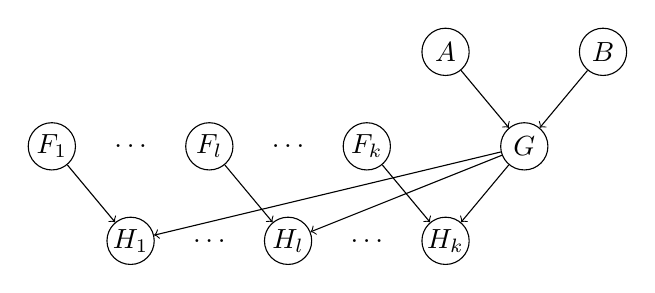
\begin{tikzpicture}[yscale=.6]
                \foreach \x/\y/\n/\t in {0/4/f1/F_1, 2/4/fl/F_l, 4/4/fk/F_k, 6/4/g/G, 1/2/h1/H_1, 3/2/hl/H_l, 5/2/hk/H_k, 5/6/a/A, 7/6/b/B}
                \node[inner sep=0mm,circle,draw,minimum size=6mm] (\n) at (\x,\y) {$\t$};
                \foreach \x/\y/\n/\t in {1/4/fdots1/\ldots, 3/4/fdots2/\ldots, 2/2/hdots1/\ldots, 4/2/hdots2/\ldots}
                \node[inner sep=0mm] (\n) at (\x,\y) {$\t$};
                \foreach \s/\t in {f1/h1, fl/hl, fk/hk, a/g, b/g, g/h1, g/hl, g/hk}
                \draw[->] (\s) -- (\t);
            \end{tikzpicture}
        \end{center}
        \caption{Before reconstruction} \label{fig:before}
    \end{figure}

    \emph{Case 1.} Suppose that there is $l$ such that $\lef(F_l) \leq \lef(G)$. If $\lef(F_l) < \lef(G)$, then $F_l$ must contain all variables $x_i, \ldots, x_j$, since otherwise either $F_l$ or $H_l$ will have smaller $\tup$ then $G$. Thus $F_l$ contains $A$. Then, we can restructure the circuit by feeding $B$ to $H_l$ instead of $G$. This does not change the value of the gate computed by $H_l$ and reduces $\out(G)$. Thus $\tup({\cal C})$ increases and we are done.

    If $\lef(F_l) = \lef(G)$, then $F_l$ still cannot have gap variables among $x_i, \ldots, x_{j-1}$ as it would contradict the minimality of $G$. Thus, $F_l$ is either a range, or it is not a range, but contain all variables $x_i, \ldots, x_{j-1}$. In the latter case again $F_l$ contains $A$. In the former case $F_l$ either contains $A$, or is contain in $G$. If $F_l$ contains $A$, we can again simplify the circuit as above. If $F_l$ is contained in $G$, we have $G=H_l$, so we can remove $H_l$ from the circuit and reduce the size of the circuit.

    \emph{Case 2.} Suppose that for all $l$ we have $\lef(F_l)>\lef(G)$. Consider $l$ such that $F_l$ has the minimal $\righ(F_l)$ (if there are several such $l$ pick among them the one with the minimal $\num(F_l)$). For convenience of notation let $l=k$. Now we restructure the circuit in the following way (see \expref{Figure}{fig:after}). We feed $F_k$ to $G$ instead of $A$. We feed $A$ to $H_k$ instead of $F_k$. We feed $H_k$ to all other $H_p$'s instead of $G$.

    \begin{figure}[ht]
        \begin{center}
            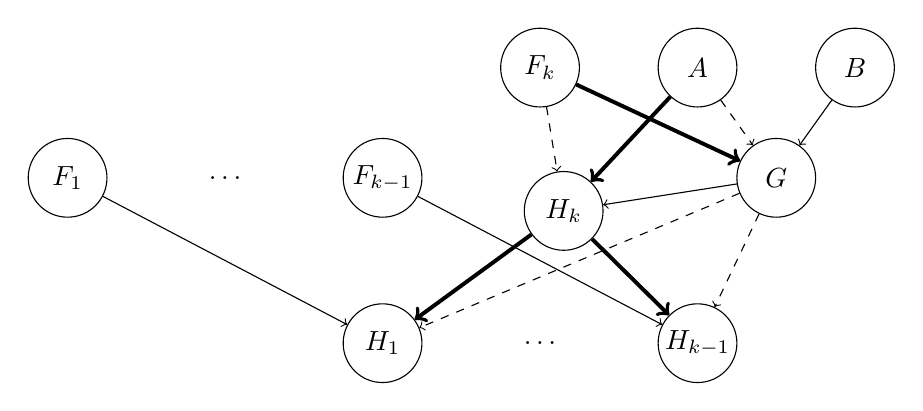
\begin{tikzpicture}[yscale=.7]
                \foreach \x/\y/\n/\t in {-3/4/f1/F_1, 1/4/fk1/F_{k-1}, 3/6/fk/F_k, 6/4/g/G, 1/1/h1/H_1, 5/1/hk1/H_{k-1}, 3.3/3.4/hk/H_k, 5/6/a/A, 7/6/b/B}
                \node[inner sep=0mm,circle,draw,minimum size=10mm] (\n) at (\x,\y) {$\t$};
                \foreach \x/\y/\n/\t in {-1/4/fdots1/\ldots, 3/1/hdots1/\ldots}
                \node[inner sep=0mm] (\n) at (\x,\y) {$\t$};
                \foreach \s/\t in {f1/h1, fk1/hk1, b/g, g/hk}
                \draw[->] (\s) -- (\t);
                \foreach \s/\t in {fk/hk, a/g, g/h1, g/hk1}
                \draw[->,dashed] (\s) -- (\t);
                \foreach \s/\t in {fk/g, a/hk, hk/h1, hk/hk1}
                \draw[->,line width=0.5mm] (\s) -- (\t);

            \end{tikzpicture}
        \end{center}
        \caption{Case 2 reconstruction} \label{fig:after}
    \end{figure}

    Observe that all these reconstructions are valid, that is, they do not create directed cycles in the circuit. To verify this we need to check that there are no cycles using new edges. Indeed, there cannot be a cycle going through one of the edges $(H_k,H_p)$ since this would mean that there was a directed path from $H_p$ to one of the vertices $F_k$, $A$ and $G$ on the original circuit. Such a path to $A$ or $G$ would mean a cycle in the original circuit. Such a path to $F_k$ violates the minimality property of $F_k$ (minimal $\righ(F_k)$). Next, there cannot be a cycle going through both edges $(F_k,G)$ and $(A,H_k)$, since substituting these edges by $(F_k,H_k)$ and $(A,G)$ we obtain one or two cycles in the original circuit. Next, there cannot be a cycle going through the edge $(A,H_k)$ only, since $H_k$ is reachable from $A$ in the original circuit and this would mean a cycle in the original circuit. Finally, there cannot be a cycle going only through the edge $(F_k,G)$ since this would mean a directed path from $G$ to $F_k$ in the original circuit and this contradicts $\lef(F_k)>\lef(G)$.

    Note that our reconstruction might require reordering of the circuit gates, since we create edges between previously incomparable $H$-gates and between $F_k$ and $G$. But the reordering affect only the gates with $\num$ greater than $\num(G)$ and may only reduce $\num(F_k)$ to be smaller than $\num(G)$. But this can only increase $\tup(G)$ and since $\lef(F_k)>\lef(G)$ this can only increase $\tup({\cal C})$.

    Observe, that the circuit still computes the outputs correctly. The changes are in the gates $H_1\ldots, H_k$ (and also in $G$, but $H_1,\ldots, H_k$ are all of its outputs). $H_k$ does not change. Other $H_p$'s might have changed, they now additionally include variables of $F_k$. But note that all of these variables are in between of $\lef(H_p)$ and $\righ(H_p)$, so they must be presented in the output gates connected to $H_p$ anyway (recall that at the output gates we compute ranges).

    Now, observe that $\tup(G)$ has increased (by the first coordinate). There are no new gates with smaller $\lef$. Among gates with the minimal $\lef$ there are no new gates with smaller $\gap$. Among gates with minimal $(\lef,\gap)$ all gates have larger $\num$ then $G$. Thus $\tup({\cal C})$ increased and we are done.  %% ToC edit1 <-- done with what?  a lemma, or a
%% main result (or both)?  Please state
\end{proof}

\section{Open problems}
There are several natural problems left open.
\begin{enumerate}
\item Design a~deterministic $O(z)$ time algorithm for generating
a~circuit in the commutative case.
For this, it suffices to design an $O(n)$ deterministic algorithm for the
following problem: given a~list of positions of $n$~zeroes of an $n \times n$
0/1-matrix with at most $\log n$ zeroes in every row, permute its columns so
that the total length of all segments of length at most $O(\log n)$ is
$O(n/\log n)$.
\item Determine the asymptotic complexity of the linear operator in terms of the number of zeroes in the non-commutative case.
\item After the preliminary version of our paper
\cite{conf-version}, %% ToC edit1 <-- inserted
Stasys Jukna posed a question on how large % can %% ToC edit1 <-- delete "can", it appears later
the gap between the complexity of the operators $Ax$ and $\overline{A}x$ can be over
the  %% ToC edit1 <-- inserted
$(\mathbb{N},+)$ semiring, where $A \in \{0,1\}^{n\times n}$ and $\overline{A}$ is
% a bit-wise  %% ToC edit1 -->
the bitwise %% <--
negation of $A$. Our result rules out the possibility of achieving
a  %% ToC edit1 <-- inserted
super-constant (multiplicative) gap with sparse matrix $A$.

\end{enumerate}


%\clearpage  %% ToC edit1 <-- removed

\appendix
\section{Review}

%% AU comment out the whole subsection
%\subsection{Algebraic structures}\label{subsec:algstr}
%
%A~\emph{semigroup} $(S, \circ)$ is an algebraic structure where the operation
%$\circ$ is \emph{closed}, \ie, $\circ : S\times S \rightarrow S$, and
%\emph{associative}, \ie,
%$x \circ (y \circ z) = (x \circ y) \circ z$ for all $x$, $y$, and $z$ in $S$.
%\emph{Commutative} (or \emph{abelian}) semigroups introduce one extra
%requirement: $x \circ y = y \circ x$ for all $x$ and $y$ in $S$.
%
%Commutative semigroups are ubiquitous. Below we list a few
%notable examples, starting with the most basic one, %% ToC edit1 what you
%%% list is not one but several semigroups with Z as their underlying set.
%which is, arguably, known to every person on the planet.  %% ToC edit1
%%% I would suggest to omit this "cute" comment.  Partly, it is undefined (which
%%% semigroup on Z are you referring to?), partly, negative numbers are not known
%%% to everyone
%
%\begin{itemize}
%\item % Integer numbers  %% ToC edit1 -->
%    The integers  %% <--
%    form commutative semigroups with many operations. For
%    example, the order in which numbers are \emph{added} is irrelevant, hence
%    $(\mathbb{Z}, +)$ is a commutative semigroup. So are $(\mathbb{Z}, \times)$,
%    $(\mathbb{Z}, \min)$ and $(\mathbb{Z}, \max)$.
%    %% ToC edit1 it is not clear who you think your audience is.
%    %% Please delete this discussion of subtraction.  -->
%    On the other hand, it does
%    matter in which order numbers are \emph{subtracted}, hence $(\mathbb{Z}, -)$
%    is not a commutative semigroup: $1-2 \neq 2-1$. In fact, $(\mathbb{Z}, -)$
%    is not even a semigroup, since subtraction is non-associative:
%    $1-(2-3) \neq (1-2)-3$.   %% <--
%
%    \item Booleans form commutative semigroups $(\mathbb{B}, \vee)$,
%    $(\mathbb{B}, \wedge)$, $(\mathbb{B}, \oplus)$ and $(\mathbb{B}, \equiv)$.
%    %% ToC edit1 please DEFINE \mathbb{B} !  ATTN1
%
%    \item Any commutative semigroup $(S, \circ)$ can be \emph{lifted} to the set
%      $\hat{S}$ of ``containers'' %% ToC edit1 this is not a "lifting" in
%      %% the usual sense, so you are redefining a common term.  In fact, you are
%      %% not defining it, just throwing in an unnecessary, undefined, and misleading
%      %% term.  You are also introducing the never-used and undefined term "container";
%      %% this only further loads the paper with unnecessary terminology.  In fact
%      %% it seems to me that you "containers" are special cases of the direct sum
%      %% why not simply say that direct sums of (commutative) semigroups are
%      %% (commutative) semigroups; examples inlcude vectors and matrices over S.
%      of elements $S$, \eg, vectors or matrices,
%    obtaining a commutative semigroup $(\hat{S}, \hat{\circ})$, where the lifted
%    operation~$\hat{\circ}$ is applied to the contents of containers
%    % element-wise.  ToC edit1 -->
%    elementwise.  %% <--
%
%    % The \cdot in \hat{\cdot} is a placeholder for an operation that is lifted
%    The lifting operation $\hat{\cdot}$ can often be omitted for clarity if there
%    is no ambiguity.
%
%    The \emph{average semigroup} $(\mathbb{Z} \times \mathbb{Z}, \circ)$ is a
%    simple yet not entirely trivial example of semigroup lifting. By defining
%    $(t_1, c_1) \circ (t_2, c_2) = (t_1 + t_2, c_1 + c_2)$, we can aggregate
%    partial \emph{totals} and \emph{counts} of a set of numbers, which allows us
%    to efficiently calculate their average as $\textit{avg}(t, c) = t/c$.
%    The average semigroup is commutative.
%
%    \item Set union and intersection are commutative and associative operations
%    giving rise to many set-based commutative semigroups. Here we highlight an
%    example that motivated our research: the \emph{graph overlay} operation,
%    %% ToC edit1 why call it "overlay"?  Why not simply "union"?  It is standard
%    %% to call this the union of graphs.  "Disjoint union" is customarily
%    %% and plausibly called just that.  I suggest to omit the discussion
%    %% of disjoint union.
%    defined\footnote{This definition coincides with that of the
%        \emph{graph union} operation~\cite{1969_graph_theory_harary}. Graph union
%        typically requires that
%the  %% ToC edit1 <-- inserted
%given graphs % are %% ToC edit1 -->
%be  %% <-- "requires" is followed by subjunctive mood
%non-overlapping, hence it is not
%        closed on the set of all graphs. Graph overlay does not have such a
%        requirement, and is therefore closed and forms a semigroup.} as
%    %% ToC edit1 the reasoning below is again kindergarden stuff, please delete
%    $(V_1, E_1) + (V_2, E_2) = (V_1 \cup V_2, E_1 \cup E_2)$,
%    % ~where~  %% ToC edit1 -->
%    where  %% <--
%    $(V, E)$ is % a %% ToC edit1 -->
%    the  %% <--
%    standard set-based representation % for %% ToC edit1 -->
%    of  %% <--
%    directed unweighted
%    % graphs, comes   %% ToC edit1 <-- this is ungrammatical -->
%    graphs.  This example comes   %% <--
%    from an algebra of graphs used in functional programming~\cite{mokhov2017algebraic}.
%    See further details in \expref{Section}{sec-dense-graph}.
%\end{itemize}
%
%\emph{Groups} % extend %% ToC edit1 -->
%restrict  %% <--
%semigroups by requiring the existence of the \emph{identity
%    element} $0 \in S$, such that $0 \circ x = x \circ 0=x$, and the \emph{inverse
%  element} $-x \in S$ for % all %% ToC edit1 it is a different inverse for each element -->
%  each  %% <--
%$x \in S$, such that
%$(-x) \circ x = x \circ (-x) = 0$. Groups provide a natural generalisation of
%arithmetic \emph{subtraction}, whereby $x \circ (-y)$ denotes the subtraction of
%$y$ from $x$.
%
%A commutative semigroup $(S, \circ)$ can often be extended to a \emph{semiring}
%$(S, \circ, \bullet)$ by introducing another associative (but not necessarily
%commutative) operation $\bullet$ that \emph{distributes} over $\circ$, that is
%\[
%x \bullet (y \circ z) = (x \bullet y) \circ (x \bullet z)\\
%\]
%\[
%(x \circ y) \bullet z = (x \bullet z) \circ (y \bullet z)
%\]
%hold for all $x$, $y$, and $z$ in~$S$. Since $\circ$ and $\bullet$~behave
%similarly to numeric addition and multiplication, it is common to give $\bullet$
%a higher precedence to avoid unnecessary parentheses, and even omit~$\bullet$~from
%formulas altogether, replacing it by juxtaposition. This gives a terser and
%more convenient notation, \eg, the left distributivity law becomes:
%$x (y \circ z) = x y \circ x z$. We will use this notation, insofar as this does
%not lead to ambiguity.
%
%Most definitions of semirings also require that the two operations have
%identities: the \emph{additive identity}, denoted by 0, such that
%$0 \circ x = x \circ 0=x$, and the \emph{multiplicative identity}, denoted by 1,
%such that $1x=x1=x$. Furthermore, 0 is typically required to be
%\emph{annihilating}: $0x=x0=0$.
%
%A semiring $(S, \circ, \bullet)$ is also a \emph{ring} if $(S, \circ)$ is a
%group, \ie, the operation $\circ$ is invertible. One can think of rings as
%semirings with subtraction.
%
%Let us extend some of our semigroup examples to
%semirings. % : %% ToC edit1 <-- (colon --> period)
%
%\begin{itemize}
%%% ToC edit1 "integer numbers" are simply called "integers" ATTN1 -->
%%% AU integer numbers -> integers (AK)
%    \item The most basic and widely known semiring is that of integers with
%    addition and multiplication: $(\mathbb{Z}, +, \times)$. Since every integer
%    number $x\in \mathbb{Z}$ has an inverse $-x \in \mathbb{Z}$ with respect to
%    the addition operation, $(\mathbb{Z}, +, \times)$ is also a ring.
%    Interestingly, integer addition can also play the role of multiplication when
%    combined with the $\max$ operation, resulting in the \emph{tropical semiring}
%    $(\mathbb{Z}, \max, +)$, which is also known as the \emph{max-plus algebra}.
%    Unlike $+$, the $\max$ operation has no inverse, therefore
%    $(\mathbb{Z}, \max, +)$ is not a ring.
%
%    \item Booleans form the semiring $(\mathbb{B}, \vee, \wedge)$. Note that
%$(\mathbb{B}, \wedge, \vee)$ is a semiring, too, %% ToC edit1 <-- commas added around "too"
%    thanks to the duality between
%    the operations $\vee$ and $\wedge$. Furthermore,
%    $(\mathbb{B}, \oplus, \wedge)$ is a ring, where every element is its own
%    inverse: $x \oplus x = 0$ for $x \in \mathbb{B}$.
%
%    \item Semirings and rings $(S, \circ, \bullet)$ can also be lifted to the set
%    $\hat{S}$ of ``containers'' of elements $S$, most commonly matrices, obtaining
%    $(\hat{S}, \hat{\circ}, \hat{\bullet})$. Matrices over tropical semirings, for
%    example, are used for solving various path-finding problems on graphs.
%\end{itemize}

%% AU queries -> query (AK)
%\subsection{Applications of the range queries problem}\label{subseq:rmqapp}
\subsection{Applications of the range query problem}\label{subseq:rmqapp}
There are many natural applications of the
%% AU queries -> query (AK)
%range queries
range query
problem for a~collection of records in a~database: computing the total population of cities that are at most some distance away from a~given point, computing an average salary in a~given period of time, finding the minimum depth on a~given subrectangle on a~sea map, etc. Below, we review some of the less straightforward applications where efficient algorithms for the
%% AU queries -> query (AK)
%range queries
range query
problem are usually combined with other algorithmic ideas.

\textbf{String algorithms and computational biology.}
It is possible to preprocess a~given string in $O(n)$ time (where $n$ is its length)
so that % to then  %% ToC edit1 -->
then to  %% <--
find the longest common prefix of any two suffixes of the original string in constant time. This is done by first constructing the suffix array and the longest common prefix array of the string and then using an efficient RMQ algorithm.

\textbf{Computational geometry.} Algorithms for the range % queries %% ToC edit1 -->
query  %% <--
%% AU problems -> problem (AK)
% problems
problem
can be used together with the scanning line technique to solve efficiently various problems like: given a~set of segments on a~line, compute the number of intersecting pairs of segments; or, given a~set of rectangles and a~set of points on a~plane, compute, for each each rectangle, the number of points it contains.

\subsection{Known approaches to range queries}\label{subsec:approaches}

In this subsection, we give a~brief overview of a~rich variety of known
algorithms for the
%% AU queries -> query (AK)
%range queries
range query
problem. We say that an algorithm has type
$(f(n), g(n))$ if it spends $f(n)$ time on preprocessing the input sequence,
and then answers any query in time $g(n)$.

\textbf{No preprocessing.} A~naive algorithm skips the preprocessing stage and
answers a~query $(l,r)$ directly in time $O(r-l+1)$. It therefore has type
$(O(1), O(n))$.

\textbf{Full preprocessing.} One may precompute the answers to all possible
queries to be able to answer any subsequent query immediately. Using dynamic
programming, it is possible to precompute the answers to all $\Theta(n^2)$
queries in time $O(n^2)$: for this, it is enough to process the queries in
order of increasing length. This gives an $(O(n^2), O(1))$ algorithm.

\textbf{Fixed length queries (sliding window).} In case one is promised that all
the queries are going to have the same length~$m$, it is possible to do
an~$O(n)$ time preprocessing and then to answer any query in time $O(1)$. For
this, one partitions the input sequence of size~$n$ into $n/m$ blocks of
size~$m$. For each block, one computes all its prefixes and suffixes in time
$O(m)$. The overall running time is $O(n/m \cdot m)=O(n)$. Then, each query
of length~$m$ touches at most two consecutive blocks and can be answered by
taking a~precomputed suffix of the left block and a~precomputed prefix of the
right block in time $O(1)$. This, in particular, implies that, given a~sequence
of length~$n$ and an integer $1 \le m \le n$, one may slide a~window of
length~$m$ through the sequence and to output the answer to all such window
queries in time $O(n)$.


\textbf{Prefix sums.} In case the semigroup operation has an \emph{easily
    computable inverse}, there is an~$(O(n), O(1))$ algorithm. We
illustrate this for a~group $(\mathbb{Z}, +)$. Given $x_1, \dotsc, x_n$, we
compute $(n+1)$ prefix sums:
\(S_0=0,\, S_1=x_1,\, S_2=x_1+x_2, \dotsc, S_n=x_1+\dotsb+x_n\,.\)
This can be done in time $O(n)$ since $S_i=S_{i-1}+x_i$. Then, the answer to any
query $(l,r)$ is just $S_r-S_{l-1}$.

Note that the algorithm above solves a \emph{static} version of the problem. For
the \emph{dynamic} version, where one is allowed to change the elements of the
input sequence, there is a~data structure known as Fenwick's
tree~\cite{DBLP:journals/spe/Fenwick94}. It allows to change any element as well
as to retrieve any prefix sum in time $O(\log n)$.

\textbf{Block decomposition.} One decomposes the input range $(1,n)$ into
$n/b$~blocks of length~$b$ and then computes, for each block, all its prefixes
and suffixes. This can be done in time $O(n)$. Then, for each query, if it lies
entirely in a~block, we compute the answer directly (hence, in time at most
$O(b)$). If it crosses a~number of blocks, we decompose it into a~suffix of
a~block, a~number of consecutive blocks, and a~prefix of a~block. This allows us
to answer such long queries in time $O(n/b)$. Setting $b=\sqrt{n}$ to balance
both cases, we get a~$(O(n), O(\sqrt{n}))$-algorithm.

\textbf{Sparse table.} This data structure works for idempotent semigroups
(\emph{bands}) and has the type $(O(n\log n), O(1))$. We illustrate its main idea
for the \emph{range minimum query} (RMQ)  (\ie, for a~semigroup
$(\mathbb{Z}, \min)$). One precomputes answers to $O(n\log n)$ queries---namely,
those whose length is a~power of~2. More formally, for all $0 \le k \le \log_2n$
and $1 \le i \le n-2^k+1$, let $S_{k,i}$ be the answer to a~query $(i, i+2^k-1)$:
\(S_{k,i}=x_i \circ x_{i+1} \circ \dotsb \circ x_{i+2^k-1} \, .\)
Since any range of length $2^k$ consists of two ranges of length $2^{k-1}$, one
can compute all $S_{k,i}$'s in time $O(n\log n)$ using dynamic programming.
Then, any range $(l,r)$ can be covered by two precomputed ranges: if $k$~is the
smallest integer such that $2^k \ge (r-l+1)/2$, then the answer to this query
is $S_{k,l} \circ S_{k,r-2^k+1}$ (idempotency is required since we are covering
the range, but not partitioning it). This gives an $(O(n\log n), O(1))$
algorithm.

\textbf{Hybrid strategy.} One may extend the block decomposition
approach further and use one efficient data structure on top of
blocks and possibly a~different data structure for each block.
Namely, we decompose the input range into blocks of size~$b$,
use a~$(p_1(n), q_1(n))$-algorithm on top of blocks and
a~$(p_2(n), q_2(n))$-algorithm within each block. The resulting algorithm then
has type
\[(O(n + p_1(n / b) + (n / b) \cdot p_2(b), O(q_1(n/b) + q_2(b))) \, .\]
For example, for the range minimum problem, combining the sparse table data
structure ($p_1(n)=O(n\log n)$, $q_1(n)=O(1)$) with no preprocessing technique
($p_2(n)=O(1)$, $q_2=O(n)$) and block size $b=\log n$, gives
an~$(O(n), O(\log n))$-algorithm. Another example: using sparse table in both
cases (with block size $b=\log n$) gives an $(O(n\log\log n), O(1))$ algorithm.

% reference: https://web.stanford.edu/class/cs166/lectures/00/Slides00.pdf

\textbf{Segment tree.} The segment tree data structure is also based on dynamic
programming ideas and works for any semigroup. Consider the following complete
binary tree with $O(n)$ nodes: the root is labelled by a~query $(1,n)$, the two
children of each inner node $(l,r)$ are labelled by the left and right halves of
the current query (\ie, $(l,m)$ and $(m+1,r)$ where $m=(l+r)/2$), the leaves
are labelled by length one queries. Going from leaves to the root, one can
precompute the answers to all the queries in this tree in time $O(n)$. Then, it
is possible to show that any query $(l,r)$ can be  partitioned into $O(\log n)$
queries that are stored in the tree. This gives an $(O(n), O(\log n))$
algorithm. It should be noted that the segment tree can also be used to solve
the dynamic version of the
%% AU queries -> query (AK)
% range queries
range query
problem efficiently: to change the
value of one of the elements of the input sequence, one needs to adjust the
answers to $O(\log n)$ queries stored in the tree.

\textbf{Algorithms by Yao and by Alon and Schieber.}
Yao~\cite{DBLP:conf/stoc/Yao82} showed that, for any semigroup, it is possible
to preprocess the input sequence in time $O(n)$ so that
% to further answer any query %% ToC edit1 -->
%% AU further -> range (AK)
%any further query can be answered %% <--
any range query can be answered %% <--
%% ToC edit1 "any further query"?  what type of queries are we talking about? ATTN1
in time $O(\alpha(n))$ where $\alpha(n)$ is the inverse Ackermann function
and proved a~matching lower bound. Later, Alon and
Schieber~\cite{Alon87optimalpreprocessing} studied a~more specific question:
what is the minimum number of semigroup operations needed at the preprocessing
stage for being able to then answer any query in at most $k$~steps? They proved
matching lower and upper bounds for every~$k$. As a~special case, they show how
to preprocess the input sequence in time $O(n\log n)$ so that % to answer
any subsequent query
can be answered %% ToC edit1 <-- inserted
by applying at most one semigroup operation. This algorithm
generalizes the sparse table data structure (as it does not require the
semigroup to be idempotent) and is particularly easy to describe. It is based on
the divide-and-conquer paradigm. Let $m=n/2$. We precompute answers to all
queries of the form $(i,m)$ and $(m+1,j)$, where $1 \le i \le m$ and
$m+1 \le j \le n$ (\ie, suffixes of the left half and prefixes of the right
half). This allows to answer in a~single step any query that intersects the
middle of the sequence, \ie, queries $(l,r)$ such that $l \le m \le r$. All the
remaining preprocessing boils down to answering queries that lie entirely in
either left or right half. This can be done recursively for the halves. The
corresponding recurrence relation $T(n)=2T(n/2)+O(n)$ implies an upper bound
$O(n\log n)$ on preprocessing time (and hence, the number of semigroup
operations).

\textbf{$(O(n), O(1))$-type algorithms.}
There is a~sequence of $(O(n), O(1))$-type algorithms designed specifically
% to %% ToC edit1 -->
for  %% <--
the range minimum query problem and a~related problem called least common
ancestor (LCA) \cite{DBLP:journals/siamcomp/BerkmanV93,
    DBLP:journals/jal/BenderFPSS05,
    DBLP:conf/latin/BenderF00,
    DBLP:conf/cpm/FischerH06}. Here, we briefly sketch the algorithm by Bender and
Farach-Colton. Its main idea is to first reduce RMQ to LCA (the least common
ancestor problem). One then reduces LCA back to RMQ and notices that the
resulting instance of RMQ has a~convenient property: the difference between any
two consecutive elements is $\pm 1$. This property allows to do the following
trick: we precompute answers to all relatively short queries (this can be done
even without knowing the input sequence because of the $\pm 1$ property); we
also partition the input sequence into blocks and build a~segment tree out of
these blocks.

%% AU comment out the whole subsection (AK)
%\subsection{Dense graph representation}\label{sec-dense-graph}
%
%Let us revisit the graph semigroup defined in \expref{Section}{subsec:algstr}.
%We will denote it by $(G_U, +)$, where $G_U$ is the set of directed graphs whose
%vertices come from a universe $U$, that is, if $(V, E) \in G_U$ then
%$V \subseteq U$ and $E \subseteq V \times V$. Recall that the graph overlay
%operation $+$ is defined as
%
%\[
%(V_1, E_1) + (V_2, E_2) = (V_1 \cup V_2, E_1 \cup E_2)\,.
%\]
%
%\noindent
%The algebra of graphs presented in~\cite{mokhov2017algebraic} also defines
%the \emph{graph connect} operation $\rightarrow$:\footnote{The definition
%    coincides with that of \emph{graph join}~\cite{1969_graph_theory_harary}, but,
%    just like graph union, graph join requires that given graphs are
%    non-overlapping. The connect operation has no such requirement.}
%
%\[
%(V_1, E_1) \rightarrow (V_2, E_2) = (V_1 \cup V_2, E_1 \cup E_2 \cup V_1 \times V_2)\,.
%\]
%
%This operation allows us to ``connect'' two graphs by adding edges from every
%vertex in the left-hand graph to every vertex in the right-hand graph, possibly
%introducing self-loops if $V_1 \cap V_2 \neq \emptyset$. The operation is
%associative, non-commutative and distributes over $+$. Note, however, that the
%empty graph $\varepsilon = (\emptyset, \emptyset)$ is the identity for both
%overlay and connect operations: $\varepsilon + x = x + \varepsilon = x$ and
%$\varepsilon \rightarrow x = x \rightarrow \varepsilon = x$, and consequently
%the annihilating zero property does not hold, which makes this algebraic
%structure not a~semiring according to the classic semiring definition.
%
%By using the two operations one can construct any graph starting from primitive
%single-vertex graphs. For example, let $U=\{1,2,3\}$ and $k$ stand for a
%single-vertex graph $({k}, \emptyset)$. Then:
%
%\begin{itemize}
%    \item $1 \rightarrow 2$ is the graph with a single edge $(1,2)$, \ie,
%    $1 \rightarrow 2 = (\{1,2\}, \{(1,2)\})$.
%    \item $1 \rightarrow (2 + 3)$ is the graph $(\{1,2,3\}, \{(1,2),(1,3)\})$.
%    \item $1 \rightarrow 2 \rightarrow 3$ is the graph $(\{1,2,3\}, \{(1,2),(1,3),(2,3)\})$.
%\end{itemize}
%
%\noindent
%Clearly any sparse graph $(V, E)$, \ie, a graph with a sparse
%% connectivity %% ToC edit1 The universally accepted term in graph theory is -->
%adjacency  %% <-- ATTN1
%matrix, can be constructed by a linear-size expression:
%
%\[
%(V, E) = \sum_{v \in V} v + \sum_{(u,v) \in E} u \rightarrow v\,.
%\]
%
%\noindent
%But what about complements of sparse graphs, \ie, graphs with dense
%connectivity matrices?  %% ToC edit1 a dense graph is usually defined as a graph
%%% whose edge density is bounded away form 0.  So a graph with edge density
%%% say 1/3 is dense, and so is its complement.  Your concept could be called
%%%  "co-sparse."    ATTN1
%It is not difficult to show that by applying the dense
%linear operator we can obtain a linear-size circuit comprising 2-input gates
%$+$ and $\rightarrow$ for any dense graph.
%
%Let $A$ be a dense matrix of size $n\times n$. Our goal is to construct the
%graph $G_A = (\{1, \dots, n\}, E)$ such that $(i,j) \in E$ whenever $A_{ij}=1$.
%
%First, we compute the dense linear operator $\mathbf{y} = A \mathbf{x}$ over the
%(commutative) graph semigroup~$+$, where $\mathbf{x} = (1, 2, \dots, n)$, \ie,
%$x_j$ is the primitive graph comprising a single vertex~$j$, obtaining
%graphs~$y_i$ that comprise sets of isolated vertices corresponding to the rows
%of matrix~$A$:
%
%\[
%y_i = \sum_{A_{ij}=1} j \, .
%\]
%
%The resulting graph $G_A = (\{1, \dots, n\}, E)$ can now be obtained by using
%the % connect  %% ToC edit1 -->
%``connect''  %% <--
%operation % ~$\rightarrow$ %% ToC edit1 -->
%``$\rightarrow$''  %% <--
%to connect $i$ to all vertices $y_i$,  %% ToC edit1 is this happening
%%% for all i simultaneously?
%and subsequently overlaying the results:
%
%\[
%G_A = \sum_{i=1}^{n} i \rightarrow y_i\,.
%\]
%
%Thanks to the linear-size construction for the dense linear operator, the size
%of the circuit computing $G_A$ is $O(n)$. This allows us to store dense graphs
%on $n$ vertices using $O(n)$ memory, and perform basic transformations of dense
%graphs in $O(n)$ time. We refer the reader to~\cite{mokhov2017algebraic} for
%further details about applications of algebraic graphs in functional programming
%languages.


\section*{Acknowledgments}
We thank
%% AU add Polish diacritics (AK)
% Pawel Gawrychowski
Pawe\l{} Gawrychowski
for pointing us to the
paper~\cite{DBLP:journals/ijcga/ChazelleR91}, and Alexey Talambutsa for
fruitful discussions on the theory of semigroups.
We are also grateful to the reviewers for their thorough reviews that helped us
improve the final version of the paper.


\bibliographystyle{tocplain}
% \bibliography{references}
\bibliography{bibstrings.bib,v021a2032,bibtail.bib}

%%% !!! AUTHOR
%%% Include a short description of each author's affiliation
%%% following the structure below. Use the same unique ID used
%%% previously (presumably lower case last name).
%%% Use \tocat{} and \tocdot{} instead of "@" and "." in emails
% \begin{tocinfo}[surname]
%     Firstname Surname\\
%     Assistant professor\\
%     Department of Computer Science and\\
%     Department of Immunology\\
%     Exemplar University\\
%     Town, State/Province, Country\\
%     name\tocat{}cs\tocdot{}exemplar\tocdot{}edu \\   %% email address here
%     \url{http://cs.exemplar.edu/~surname}      %% your home page here
%    \end{tocinfo}

\begin{tocauthors}
\begin{tocinfo}[kulikov]
    Alexander S. Kulikov\\
    Steklov Mathematical Institute at St.~Petersburg,     Russian Academy of~Sciences\\ and St.~Petersburg State University\\
    kulikov\tocat{}logic\tocdot{}pdmi\tocdot{}ras\tocdot{}ru\\
    \url{https://alexanderskulikov.github.io/}
\end{tocinfo}
\begin{tocinfo}[mikhailin]
    Ivan Mikhailin\\
    Steklov Mathematical Institute at St.~Petersburg,     Russian Academy of~Sciences\\
    ivmihajlin\tocat{}gmail\tocdot{}com
\end{tocinfo}
\begin{tocinfo}[mokhov]
    Andrey Mokhov\\
    Jane Street Singapore\\
    and School of Engineering, Newcastle University, United Kingdom\\
    andrey.mokhov\tocat{}ncl\tocdot{}ac\tocdot{}uk
\end{tocinfo}
\begin{tocinfo}[podolskii]
    Vladimir V. Podolskii\\
    Tufts University\\
    and Steklov Mathematical Institute, Russian Academy of Sciences\\
    vladimir.podolskii\tocat{}tufts\tocdot{}edu\\
\end{tocinfo}
\end{tocauthors}

%% ToC edit1 please add bio sketches.  It seems you erased the instructions, please
%% find them in the template.  Also there are models in every published ToC article.
%% Please include advisors, dates, links, possibly pay tribute to an early and influential
%% mentor.  Some humor is welcome.
%% AU added bio sketches
\begin{tocaboutauthors}
\begin{tocabout}[kulikov]
  \textsc{Alexander Kulikov}  %% add bio sketch
  holds PhD and DrSci degrees from St.~Petersburg Department of Steklov Mathematical Institute. His scientific interests include algorithms, circuit complexity, and Computer Science education. In~his spare time, he~enjoys discussing circuit complexity of the $\operatorname{MOD}_3$ function with Alexander Golovnev.
\end{tocabout}
\begin{tocabout}[mikhailin]
  \textsc{Ivan Mikhailin}    %% add bio sketch
  is a~researcher at JetBrains Research.
  His research areas are circuit complexity,
  fine-grained complexity, and algorithmic theory.
\end{tocabout}
\begin{tocabout}[mokhov]
  \textsc{Andrey Mokhov}    %% add bio sketch
  is~a~software engineer at~Jane Street Singapore, and
  a~visiting fellow at~Newcastle University, UK. His research interests are in
  applying abstract mathematics and functional programming to solving large-scale engineering problems. During his PhD (2005--2009), Andrey worked
  on asynchronous circuits and concurrency theory. In~2014, he~became interested in functional programming and software build systems, which
  eventually led him to writing more and more code, and in~2019, he switched from academia to~industry, joining Jane Street's Tools and Compilers
  team. Andrey is~originally from Kyrgyzstan where he~helps to~run the ACM ICPC regional programming contest.
\end{tocabout}
\begin{tocabout}[podolskii]
  \textsc{Vladimir Podolskii}   %% add bio sketch
  defended his PhD thesis in~2009 at~Moscow State University. His research areas are circuit complexity, its applications to~databases augmented with ontologies, min-plus algebra. He is an Associate Professor at Tufts.
\end{tocabout}
\end{tocaboutauthors}

\end{document}
